% $Id$
\documentclass[10pt]{article}
\usepackage{epsfig}
\usepackage{dcolumn}
\usepackage{alltt}

\def\numpackages{30}
\def\numpackageslesstwo{28}
\def\numlines{2 million}
\def\numlinesexact{nearly 2 million}
\def\numlinesalmost{almost 2 million}
\def\numlinesncnbexact{about 1.4 million}

% ``article'' or ``report''
\def\typeofdocument{article}

\newcommand{\pkg}[1]{\textsf{#1}}

\newcommand{\file}[1]{\texttt{#1}}

% the "fullpage" package does almost the same thing
% as the below lines-- it doesn't make things quite as
% tall or wide, but is generally what I use
% \usepackage{fullpage}
\marginparwidth 0pt
\oddsidemargin  0pt
\evensidemargin 0pt
\marginparsep 0pt
\topmargin   0pt
\headsep 0pt
\headheight 0pt
\textwidth   6.5 in
\textheight  9 in

%% Figures
\newcommand{\captionsmall}[1]{\caption[]{\small #1}}
% Changing this to .9 shoves lots of figures to the end of the document; why?
\renewcommand{\floatpagefraction}{.8} %default .5
% \renewcommand{\floatpagefraction}{.9} %default .5
% Avoid putting all figures at end of text.
\renewcommand{\textfraction}{.1}  % .2 is the default
\renewcommand{\topfraction}{.9}   % .7 is the default
%% Get a line between figures at the top of the page and the text
 \makeatletter
 \def\topfigrule{\kern3\p@ \hrule \kern -3.4\p@} % the \hrule is .4pt high
 \def\botfigrule{\kern-3\p@ \hrule \kern 2.6\p@} % the \hrule is .4pt high
 \makeatother


%%% end of header
%%%%%%%%%%%%%%%%%%%%%%%%%%%%%%%%%%%%%%%%%%%%%%%%%%%%%%%%%%%%%%%%%%%%%%%%%%%

\begin{document}
% \bibliographystyle{plain}
\bibliographystyle{alpha}

\title{An Empirical Analysis of C Preprocessor Use}

\author{Michael D. Ernst \and Greg J. Badros \and David Notkin}

\date{% Technical Report UW-CSE-97-04-06 \\
Department of Computer Science and Engineering \\
University of Washington \\
Box 352350, Seattle, WA  98195-2350  USA \\
{\small \{{\tt mernst},{\tt gjb},{\tt notkin}\}{\tt @cs.washington.edu}} \\
28 November 1997}  

\maketitle

\begin{abstract}
  The C programming language is intimately connected to its macro
  preprocessor, Cpp.  This relationship hinders tools built to engineer C
  programs, such as compilers, debuggers, call graph extractors, and
  translators.  Most tools make no attempt to analyze macro usage, but
  simply preprocess their input, which has a number of negative
  consequences; an analysis that takes Cpp into account is preferable.  In
  order to determine how the preprocessor is used in practice, and the
  feasibility of automatic analysis of preprocessor use, this paper
  analyzes {\numpackages} packages comprising {\numlinesalmost} lines of publicly
  available C code.  We determine the incidence of C preprocessor
  usage\,---\,whether in macro definitions, macro uses, or dependences upon
  macros\,---\,that is complex, potentially problematic, or inexpressible
  in terms of other C or C++ language features.  We taxonomize these
  various aspects of preprocessor use and particularly note data that are
  material to the development of tools for C or C++, including translating
  from C to C++ to reduce preprocessor usage.  Our results show that while
  most Cpp usage follows fairly simple patterns, an effective program
  analysis tool must address the preprocessor in order to be effective.
  These results are of interest to language designers, tool writers,
  programmers, and software engineers.
\end{abstract}

\bigskip

\section{Introduction}

The C programming language~\cite{KernighanR88,Harbison91} is incomplete
without its macro preprocessor, Cpp.  By supplying such facilities as file
inclusion, definition of constants and macros, and conditional compilation,
Cpp can define new syntax, abbreviate repetitive or complicated constructs,
or eliminate reliance on a compiler implementation to inline functions,
propagate symbolic constants, eliminate dead code, and short-circuit
constant tests.  Cpp also permits system dependences to be made explicit
and tested, resulting in a clearer separation of concerns.  In addition,
Cpp permits a single source to contain multiple different dialects of C,
such as supporting both K\&R-style and ANSI-style declarations.  Indeed,
one cannot write practical C programs without these facilities.

While disciplined use of the preprocessor can reduce programmer effort
and improve portability, performance, or readability, Cpp is widely
viewed as a source of difficulty for understanding and modifying C
programs.  Cpp's lack of structure\,---\,it's inputs and
outputs are raw token streams\,---\,engenders flexibility but allows
arbitrary source code manipulations that complicate 
understanding of the program by both software engineers and tools.  In
the worst case, the preprocessor makes merely determining the program
text as difficult as determining the output of an ordinary program.
The designer of the C++ language, which shares C's preprocessor, also noted these
problems: ``Occasionally, even the most extreme uses of Cpp are
useful, but its facilities are so unstructured and intrusive that they
are a constant problem to programmers, maintainers, people porting
code, and tool builders''~\cite[p.~424]{Stroustrup-DesignEvolution}.

Tools\,---\,and, to a lesser degree, software engineers\,---\,have
three options for coping with Cpp.  They may ignore preprocessor
directives altogether, accept only post-processed code (usually by
running Cpp on their input), or attempt to emulate the preprocessor.
Each approach has different strengths and weaknesses.

\begin{itemize}

\item Ignoring preprocessor directives is an option for tools that produce
  approximate information, such as those based on lexical or approximate
  parsing techniques.  However, if accurate information about function
  extents, scope nesting, declared variables and functions, and other
  aspects of a program is required, the preprocessor cannot be ignored.

\item Operating on post-processed code, the most common strategy, is
  simple to implement, but the tool's input differs from what the
  programmer sees.  Even when line number mappings are maintained, other
  information is lost in the mapping back to the original source code.
  Source-level debuggers have no symbolic names or types for constants and
  functions introduced via {\tt \#define}, nor can tools trace or set
  breakpoints in function macros, as they can for ordinary functions (even
  those that have been inlined~\cite{Zellweger83:TR}).  Siff and Reps use
  type inference to produce C++ function templates from C; however, the
  input is ``a C program component that $\ldots$ has been preprocessed so
  that all include files are incorporated and all macros
  expanded''~\cite[p.~145]{Siff-fse96}.  Such preprocessing may limit the
  readability and reusability of the resulting C++ templates.  Call graph
  extractors generally work in terms of the post-processed code, even when
  a human is the intended consumer of the call graph~\cite{Murphy-icse18}.
  Some tools even leave the software engineer responsible for inferring the
  mapping between the original and the post-processed source, which is an
  undesirable and error-prone situation.
  
  A tool that manipulates post-processed code cannot be run on a
  non-syntactic program or one that will not preprocess on the platform on
  which the tool is being run.  These constraints complicate porting and
  maintenance, two of the situations in which program understanding and
  transformation tools are most likely to be needed.  Additionally, a tool
  supplied with only one post-processed instantiation of the source code
  cannot reason about the program as a whole, only about that version that
  results from one particular set of preprocessor variables.  For instance,
  a bug in one configuration may not be discovered despite exhaustive
  testing of other configurations that do not incorporate particular code
  or do not admit particular execution paths.

\item The final option, emulating the preprocessor, is fraught with
  difficulty.  Macro definitions consist of complete tokens but need not be
  complete expressions or statements.  Conditional compilation and
  alternative macro definitions lead to very different results from a
  single original program text.  Preprocessing adds complexity to an
  implementation, which must trade off performing preprocessing against
  maintaining the code in close to its original form.  Extracting structure
  from macro-obfuscated source is not a task for the faint-hearted.
  Despite these problems, in many situations only some sort of
  preprocessing or Cpp analysis can produce useful answers.

\end{itemize}

%All three approaches would be unnecessary if programs did not use
%preprocessor directives.  This is exactly what Stroustrup suggests:
%\begin{quote}
%  I'd like to see Cpp abolished.  However, the only realistic and
%  responsible way of doing that is first to make it redundant, then
%  encourage people to use the better alternatives, and {\em then\/}\,---\,years
%  later\,---\,banish Cpp into the program development environment with the
%  other extra-linguistic tools where it
%  belongs~\cite[p.~426]{Stroustrup-DesignEvolution}.
%\end{quote}
%C++ contains features\,---\,such as constant variables, inline functions,
%templates, and reference parameters\,---\,that obviate many uses of Cpp.
%Thus, translation to C++ is a path for partial elimination of Cpp.
%This study indicates the
%feasibility\,---\,and our framework for analyzing preprocessor usage
%provides a basis for the development\,---\,of an automatic translator with
%two attractive properties.  It would take as input C programs complete with
%preprocessor directives, and it would map many uses of directives into C++
%language features.  (It is not 
%practical to eliminate all uses of Cpp.  For example, C++ currently
%provides no replacement for the {\tt \#include} directive, or for
%stringization or pasting.  Macros that cannot be eliminated might be
%annotated with their types or 
%effects on parser or program state, so that even tools that do no Cpp
%analysis can operate correctly on such programs.)

Choices among these options are made in the absence of
an understanding of how Cpp is used in practice.
While  Cpp's potential pitfalls are well-known, no
previous work has examined actual use of the C preprocessor to
determine whether it presents a practical or merely theoretical
obstacle to program understanding, analysis, and modification.  This
paper fills that gap by examining Cpp use in {\numpackages} programs
comprising {\numlines} lines of source code.

The analysis focuses on potential pitfalls that complicate the work of
software engineers and tool builders:
\begin{description}\itemsep 0pt \parskip 0pt
\item[high total use]  Heavy use of either macro substitution or
  conditional compilation can overwhelm a human or tool.  Particularly
  problematic are lines that depend on many macros or macros that control
  many lines.
\item[complicated bodies]  A macro body need not expand to a complete
  C syntactic entity (like a statement or expression).
\item[extra-linguistic features]  a macro body may exploit features of
  the preprocessor not available in C, such as stringization, token
  pasting, or use of free variables.
\item[multiple definitions]  Uncertainty about the expansion of a macro
  prevents knowledge of the actual program text.  Even more problematically,
  two definitions of a macro may be incompatible, for instance if one is a
  statement and the other expands to an expression or type.
\item[macro pitfalls]  Macros introduce new varieties of programming
  errors, such as function-like macros that fail to swallow a following
  semicolon and macros that fail to parenthesize, or side-effect, uses of
  formal variables.
\item[inconsistent usage]  A macro used both for conditional compilation
  and to expand code is harder to understand than one used just for one
  purpose.
\item[mixed tests]  A single Cpp conditional may test conceptually
  distinct, unrelated conditions, making it difficult to perceive the
  test's purpose.
\item[variation in use]  In the absence of a clear pattern of use or
  commonly-repeated paradigms, no obvious point of attack presents itself
  to eliminate most complexity with little effort.
  %% No pattern according to package size, relative or absolute Cpp use, etc.
\end{description}

We report in detail on each of these aspects of preprocessor use,
indicating which are innocuous in practice and which problematic
uses appear more frequently.  We also present new taxonomies of macro body
expansions, macro feature usage, macro pitfalls, and conditional
intentions.  These taxonomies improve on previous work by being more
detailed and more accurately reflecting actual use.

Overall, our analysis confirms that the C preprocessor is used in
exceptionally broad and diverse ways, complicating the development of C
programming support tools.  By far the largest number of macro definitions
and uses are relatively simple, of the variety that a programmer could
understand through simple but tedious effort or that a relatively
unsophisticated tool could understand (although in practice very few even
try).  Despite the preponderance of innocuous macros, the preprocessor is
so heavily used that the remaining ones, which are most likely to cause
difficulties, are numerically significant, so understanding, annotating, or
eliminating them is worthwhile.

Section~\ref{sec:methodology} describes our experimental methodology.
Sections~\ref{sec:first-content-section}--\ref{sec:last-content-section}
present the bulk of results about macro preprocessor use.
Section~\ref{sec:related} discusses related work, and
Section~\ref{sec:easier-to-understand} suggests techniques for mitigating
the negative impact of Cpp on program understanding.
Section~\ref{sec:conclusion} discusses the relevance of the research and
discusses avenues for future work.

%[[Point reader at conclusion/summary of results, at end of paper (and write
%that!).]]

% \subsection{Outline}
% 
% The remainder of this paper is organized as follows.
% 
% Section~\ref{sec:directives} reports the percentage of original C source
% code lines that are preprocessor directives, including a breakdown of the
% frequency of specific directives such as {\tt \#define}.  C programs
% commonly have preprocessor directives as over 10\% of their total lines,
% and over 20\% of the lines are directives in 3 of the {\numpackages}
% packages.
% 
% Section~\ref{sec:usage} reports how often each macro is defined and
% expanded.   Identifiers tend to be {\tt \#define}d relatively few times
% (96\% of macro identifiers have three or fewer definitions).  Many packages
% also have a significant number of macros that are never expanded, even
% disregarding system and library header files.
% 
% Section~\ref{sec:categorization} categorizes macro definitions according to
% their expansions; for example, macros may simply define a preprocessor
% symbol, define a literal, expand to a statement, etc.  We were particularly
% interested in determining the frequency of use of macros that are difficult
% to convert to other language features, such as those that string together
% characters as opposed to manipulating lexemes or syntactic units (less than
% one third of one percent of all macro definitions),
% those that expand to partial syntactic units such as unbalanced
% braces or partial declarations (half of one percent), and others not 
% directly expressible in the programming language (about four percent).
% 
% Section~\ref{sec:conclusion} discusses the relevance of the research,
% suggests techniques for mitigating the negative impact of Cpp on program
% understanding, and discusses avenues for future work, while
% Section~\ref{sec:related} discusses related work.


%[[Does anyone care about this?
%Another niche already filled by our tool is that of a ``macro lint''
%program which warns of potentially dangerous (or non-standard) uses of Cpp.
%And, we wrote Cppp.]]



%Overall, our analysis confirms that the C preprocessor is used in
%exceptionally broad and diverse ways, complicating the development of C
%programming support tools.  On the other hand, the analysis also convinces
%us that, by extending our analysis framework with some class type
%inferencing techniques (similar to those used for C to C++
%translation~\cite{Siff-fse96} and for program
%understanding~\cite{OCallahan-icse97}), we can take significant
%steps towards a tool that usefully converts a high percentage of Cpp code
%into C++ language features.  We are interested not in translations
%that merely allow a C program to be compiled by a C++ compiler (which is
%usually easy, by intentional design of C++) but those that take advantage
%of the added richness and benefits of C++ constructs.
%

%
%[[Where do these two points go?]]
%
%Another niche already filled by our tool is that of a ``macro lint''
%program which warns of potentially dangerous (or non-standard) uses of Cpp.
%
%And, we wrote Cppp.

%O'Callahan and Jackson also use type
%inference, although for program understanding rather than translation;
%they, too, apply their techniques to post-processed
%code~\cite{OCallahan-icse97}.


%%% NEED A REFERENCE TO DEBUGGER HERE!
%%% also mention Emacs hide-ifdef mode

%Our long-term goal is not to take these useful features away from
%programmers, but to reduce Cpp use, making programs easier for humans to
%understand and tools to analyze.


\section{Methodology}
\label{sec:methodology}

We analyzed {\numpackages} publicly-available software packages that
represent a mix of application domains, authors, programming styles, and
sizes.  Some are interactive, while others are not; some are graphical,
while others are text-based command-line applications.
Figure~\ref{fig:packages} describes the packages and lists their sizes in
terms of physical lines (newline characters) and non-comment, non-blank
(NCNB) lines.  The NCNB figure disregards lines consisting of only comments
or whitespace, as well as lines in a conditional that cannot evaluate to
true (such as {\tt \#if 0}, which is frequently used to comment out code).
The remainder of our analysis uses the NCNB length, which more accurately
reflects the amount of source code.

\begin{figure}
\centering
{% ``\small'' here does have an effect, despite previous comment to the contrary
  \small
  \setlength{\tabcolsep}{.25em}
  \begin{tabular}{|l|r|r|r|r|l|}\hline
Package & Version & Physical lines & NCNB lines & Files & Description\\\hline\hline
bash & 1.14.7 & 67,604 & 46,110 & 151 & Command shell \\\hline
bc & 1.03 & 7,483 & 5,184 & 28 & Desktop calculator \\\hline
bison & 1.25 & 11,434 & 7,676 & 33 & Parser generator \\\hline
cvs & 1.9 & 79,670 & 53,431 & 208 & Revision control system \\\hline
dejagnu & 1.3 & 64,650 & 40,286 & 150 & Testing framework \\\hline
emacs & 19.34 & 206,309 & 134,251 & 445 & Text editor\\\hline
flex & 2.5.3 & 18,969 & 13,289 & 32 & Scanner generator \\\hline
fvwm & 2.0.43 & 55,584 & 42,498 & 151 & Window manager \\\hline
g77 & 0.5.18 & 133,366 & 98,980 & 232 & Fortran compiler \\\hline
gawk & 2.15.6 & 27,705 & 18,567 & 61 & GAWK interpreter \\\hline
gcc & 2.7.2.1 & 500,752 & 324,620 & 706 & C and C++ compiler\\\hline
genscript & 1.3.2a & 12,049 & 8,166 & 32 & Text-to-PostScript converter \\\hline
ghostview & 1.5 & 11,535 & 8,897 & 23 & PostScript previewer \\\hline
gnuchess & 4.0pl77 & 30,090 & 18,538 & 41 & Chess player \\\hline
gnuplot & 3.50.1.17 & 38,209 & 29,582 & 59 & Graph plotter \\\hline
groff & 1.10 & 68,872 & 60,054 & 162 & Text formatter \\\hline
gs & 262 & 77,695 & 56,378 & 309 & PostScript interpreter \\\hline
gzip & 1.2.4 & 9,067 & 5,774 & 34 & File compressor \\\hline
m4 & 1.4 & 16,778 & 10,327 & 28 & Macro expander \\\hline
mosaic & 2.6 & 126,026 & 79,753 & 289 & WWW browser\\\hline
perl & 5.003 & 66,856 & 57,450 & 88 & Perl interpreter \\\hline
plan & 1.5.3 & 23,826 & 18,870 & 68 & Schedule planner \\\hline
python & 1.4 & 82,466 & 62,137 & 221 & Python interpreter \\\hline
rasmol & 2.5 & 27,218 & 22,109 & 27 & Molecular visualization\\\hline
rcs & 5.7 & 17,979 & 11,843 & 28 & Revision control system \\\hline
remind & 3.00.15 & 18,222 & 13,130 & 41 & Schedule reminder \\\hline
workman & 1.3 & 13,419 & 9,653 & 24 & Audio CD player \\\hline
xfig & 3.1.4 & 53,244 & 42,020 & 120 & Drawing program \\\hline
zephyr & 2.0.4 & 42,665 & 29,118 & 242 & Notification system \\\hline
zsh & 3.0.1 & 46,197 & 35,377 & 43 & Command shell \\\hline
\hline
Total & & 1,955,939 & 1,364,068 & 4,076 & 30 packages\\\hline
\end{tabular}

%%% Local Variables: 
%%% mode: latex
%%% TeX-master: t
%%% End: 

}
\captionsmall{Analyzed packages and their sizes.  NCNB lines are non-comment,
  non-blank lines.}
\label{fig:packages}
\end{figure}

Before performing our analysis, we ran {\tt configure} or the equivalent on
each package in order to prepare it for compilation.  This creates various
header files such as \file{configure.h}.  Our analysis works in the
absence of this step, but warns about uses of never-defined macros and
under-reports some values related to those missing definitions.  We did
not, however, compile the packages; our analysis does not require that the
package be compilable, or even that the preprocessor be able to run on it.

We generated a list of all the C files in the package (both code and header
files).  In general, these have extensions like \file{.c}, \file{.h},
\file{.cc}, \file{.cpp}, \file{.hxx}, etc.  We removed files with such
extensions that don't actually contain valid C, and added others that were
{\tt \#include}d by valid C files (some included files have extension
\file{.def}).

We analyzed all the C files in the package, as well as every file {\tt
\#include}d by any of those, primarily library header files.  We
took care to include as many libraries as possible so as not to overlook
those definitions.  However, the figures reported in this paper always omit
all macros defined only in libraries, as well as all macro uses in
libraries.  This prevents libraries from swamping the characteristics of
the package code, which is our focus in this study.  The programmer
generally has no control over libraries and their header files, and may not
even know whether a library symbol is defined as a macro or a true function
or variable.  Finally, we assume that library macros are carefully written
to behave correctly and robustly.  (This is not always true in practice,
but an analysis of library macros is outside the scope of this
\typeofdocument).

Our analysis is a true whole-program analysis; rather than preprocessing the
code and examining just one configuration, we examine all possible code and
ignore no possible  conditional compilation conditions (though we do skip
over those that can be statically proven to be false).   As a result, this
analysis is more thorough than traditional ``whole-program'' analyses.

% [[We merge different Cpp branches in the code wherever possible.  Discuss
% this a bit.]]

We performed our analysis via a collection of Perl scripts, totaling
approximately 11,000 lines (7,000 NCNB lines).  We perform approximate
parsing because the input may not be a valid C program; as a result, we
misinterpret some constructs, but we can cope with uncompilable C and with
partial constructs in conditional compilation branches.  Our tool includes
parsers for expressions, statements, and declarations.  The raw data, which
includes considerable data not reported here, and the programs used to
generate and manipulate them, are available from the authors.


\section{Occurrence of preprocessor directives}
\label{sec:directives}
\label{sec:first-content-section}

Figure~\ref{fig:directives-breakdown} shows how often preprocessor
directives appear in the packages we analyzed.  Each group of bars in the
figure represents the percentage of NCNB lines
attributed to the specified category of directives, with each individual
bar showing the percentage for a specific package.  Conditional compilation
directives ({\tt \#if}, {\tt \#ifdef}, {\tt \#ifndef}, {\tt \#else}, {\tt
\#elif}, {\tt \#endif}) are grouped together.

\begin{figure}
\centerline{\epsfig{file=fig/directives-breakdown.eps,height=7.5in}}
\captionsmall{Preprocessor directives as a fraction of non-comment,
  non-blank (NCNB) lines.  For
  example, 2.0\% of gzip's NCNB lines are {\tt \#include}s, and 4.4\% of all
  lines across the packages are conditional compilation directives.}
\label{fig:directives-breakdown}
\end{figure}

The prevalence of, and variation in, preprocessor use makes understanding
Cpp constructs crucial to program analysis.  Nearly one in ten program
lines is a 
preprocessor directive rather than C code.  Across packages, the percentage
varies from less than 4\% to more than 22\%.  (These figures do not include
the 28\% of lines that expand a macro or the 38\% of lines whose inclusion
is controlled by {\tt \#if}; see Section~\ref{sec:dependence}.)

% \#if 46\%, \#define 35\%, \#include 13\%, \#undef 3\%, \#line 2\%

Conditional compilation directives account for just under half (46\%) of
the total directives in all packages, macro definitions comprise another
35\%, and file inclusion makes up most of the rest.  Packages are not very
uniform in their mix of preprocessor directives, however.  (If they were,
each group of bars in figure Figure~\ref{fig:directives-breakdown} would be
a scaled version of the top group.)  In particular, the prevalence of {\tt
\#include} is essentially independent of incidence of other directives.
The percentage of directives that are conditionals varies from 16\% to
74\%, the percentage of {\tt \#define} varies from 14\% to 52\%, and the
percentage of {\tt \#include} varies from 4\% to 60\%.  This variation in
usage indicates that a tool for understanding Cpp cannot focus on just a
subset of directives.


\subsection{{\tt \#line}, {\tt \#undef}, and other directives}

The definedness of a macro is often used as a boolean value.  However, {\tt
\#undef} is rarely used to set such macros to false.  Most uses of
{\tt \#undef} immediately precede a definition of the just-undefined macro,
to avoid preprocessor warnings about incompatible macro redefinitions.

Every use of {\tt \#line} (in \pkg{bash}, \pkg{cvs}, \pkg{flex}, \pkg{fvwm},
\pkg{gawk}, \pkg{gcc}, \pkg{groff}, and \pkg{perl}) appears in lex or yacc
output that enables packages to build on systems lacking lex, yacc, or
their equivalents.  For instance, \pkg{flex} uses itself to parse its
input, but also includes an already-processed version of its input
specification (that is, C code corresponding to a {\tt .l} file) for
bootstrapping.

% , as are ``other'' directives (such as ).  
% as well as user-defined ones like {\tt \#module}

Rarely-appearing directives such as {\tt \#pragma}, {\tt \#assert}, and
{\tt \#ident}, and unrecognized directives, are omitted from
Figure~\ref{fig:directives-breakdown}.  Among the packages we studied,
these directives account for .017\% of directives, or one in six thousand.
Their only significant user is \pkg{g77}, which contains 154 uses of {\tt
\#error} (representing 1.5\% of its preprocessor directives and 0.16\% of
its NCNB lines) to check for incompatible preprocessor flags.  We ignore
the null command (``{\tt \#}'' followed by only whitespace), which produces
no output.


\subsection{Packages with heavy preprocessor use}

The \pkg{gzip}, \pkg{remind}, and \pkg{bash} packages deserve
special attention for their heavy preprocessor usage\,---\,22\%, 21\%, and
16\%, respectively.

\pkg{gzip} {\tt \#define}s disproportionately many macros as literals and
uses them as arguments to system calls, enumerated values, directory
components, and more.  These macros act like {\tt const} variables.
\pkg{gzip} also contains many conditional compilation directives, since
low-level file operations (such as setting creation time and access control
bits, accessing directories, and so forth) are done differently on
different systems.

\pkg{remind} supports speakers of multiple natural languages by using {\tt
\#define}d constants for basically all user output.  It also contains
disproportionately many conditional compilation directives; over half of
these test the definedness of \verb|HAVE_PROTO|, in order to provide both
K\&R and ANSI prototypes.

Like \pkg{gzip}, \pkg{bash} is portable across a large variety of
systems, but \pkg{bash} uses even more operating system services.
Ninety-seven percent of \pkg{bash}'s conditional compilation directives
test the definedness of a macro whose presence or absence is a boolean
flag indicating whether the current system supports a specific feature.
The presence or absence of a feature requires different (or sometimes
additional) system calls or other code.


\section{Macro definition bodies}
\label{sec:categorization}

This section examines features of macro definitions that may complicate
understanding the containing program.  These include macro definitions that
expand to a partial or unidentifiable syntactic entity, take advantage of
Cpp features that lie outside the programming language, or contain other
error-prone constructs.  Multiple definitions of a macro name can also
complicate understanding, whether the redefinitions do effectively the same
thing or have incompatible bodies.

Our tool classified over 98\% of macros, though not all of these will be
easy to understand.  Three quarters of macros correspond to complete
syntactic entities in the C language; these macros should present little
difficulty.  One sixth of macros use Cpp features unavailable in C, and one
quarter contain latent bugs.  These numbers indicate the necessity and
difficulty of a thorough understanding of macro definitions to a software
engineer or tool.  Multiple definitions of a macro are generally innocuous:
only 2\% of macros contained definitions with different abstract syntax
trees.



\subsection{Macro body categorization}

We categorized macro bodies into 28 categories, though for simplicity of
presentation, this paper coalesces these into ten higher-level categories.
We started with a set of categories that we expected to occur frequently
(similar to other macro
taxonomies~\cite{Stroustrup-DesignEvolution,Carroll95}), then iteratively
refined them to break up overly broad categories or add unforeseen ones.

Figure~\ref{fig:categorization} reports, for each package, how many
definitions create an expansion which falls in each category.  Macros that
act like C language constructs\,---\,such as variables or
functions\,---\,are easiest to analyze, understand, and perhaps even
translate into other language constructs.  Thus, there is reason to believe
that the 70\% of macros whose bodies are expressions and the 6\% that are
statements can be handled relatively easily by people and tools.  Other
macros, especially those that do not expand to a complete syntactic
construct, are more problematic.


The ten categories are as follows.  

% The examples are chosen for clarity and brevity from the packages studied.

% Where does this go?
% There's no pattern, again.  (Nor is there a pattern by package size
% or by type of application.)

% The following isn't quite enough to get the columns lined up in this table.
% \newcolumntype{d}{D{.}{.}{2}}
% \begin{tabular}{|l|d|d|d|d|d|d|d|}\hline
\begin{figure}
% {\small
%   \setlength{\tabcolsep}{.25em}
%   \centerline{\begin{tabular}{|l|c|c|c|c|c|c|c|}\hline
Package & Null define & Literal & Expression & Statement & Stringization and pasting & Other syntatic macros & Failed classification\\\hline
Python & 176 & 510 & 865 & 50 & 5 & 62 & 21\\\hline
bash & 717 & 679 & 637 & 3 & 3 & 62 & 30\\\hline
bc & 4 & 36 & 37 & 2 & 0 & 9 & 1\\\hline
bison & 4 & 64 & 32 & 0 & 0 & 2 & 0\\\hline
cvs & 106 & 683 & 530 & 58 & 0 & 69 & 116\\\hline
flex & 32 & 224 & 87 & 19 & 0 & 36 & 2\\\hline
fvwm & 48 & 748 & 122 & 11 & 0 & 27 & 1\\\hline
gawk & 49 & 243 & 391 & 11 & 0 & 59 & 23\\\hline
genscript & 8 & 71 & 39 & 0 & 0 & 9 & 0\\\hline
gnuchess & 12 & 201 & 93 & 5 & 0 & 5 & 1\\\hline
gnuplot & 134 & 577 & 244 & 3 & 0 & 18 & 9\\\hline
groff & 18 & 607 & 148 & 11 & 1 & 36 & 98\\\hline
gzip & 110 & 229 & 130 & 25 & 0 & 21 & 4\\\hline
m4 & 36 & 83 & 272 & 26 & 0 & 62 & 1\\\hline
plan & 9 & 208 & 43 & 4 & 0 & 4 & 2\\\hline
rcs & 15 & 54 & 80 & 14 & 0 & 18 & 3\\\hline
remind & 11 & 744 & 108 & 65 & 0 & 18 & 2\\\hline
workman & 1 & 41 & 25 & 2 & 0 & 0 & 0\\\hline
xfig & 31 & 681 & 240 & 24 & 0 & 20 & 0\\\hline
zephyr & 80 & 451 & 255 & 28 & 0 & 27 & 2\\\hline
zsh & 31 & 520 & 267 & 20 & 0 & 40 & 5\\\hline
\hline
Total & 1632 & 7654 & 4645 & 381 & 9 & 604 & 321\\\hline
\end{tabular}}%
% }
\centerline{\epsfig{file=fig/def-categories.eps,height=6in}}
\captionsmall{Categorization of macro definition bodies.  The legend numerically
  represents the information in the top row; the category names in the
  legend should be read across, by rows.}
\label{fig:categorization}
\end{figure}



\label{sec:categorization-details}

\begin{description}
  \sloppy
  \emergencystretch=2em

%%  mcat_NULL: 5391
%%    100%  null_define (5391)
% @mcat_NULL = qw( catNULL_DEFINE );
\item[Null define]  The {\tt \#define} directive gives only an
  identifier name but no macro body, as in {\tt \#define
  \verb|HAVE_PROTO|}\@.  Such macros frequently act as boolean variables in
Cpp conditionals.  In code, they often represent optional syntax.  For
instance, macro {\tt private} may expand either to {\tt static} or to
nothing, depending on whether a debugging mode is set.

%%  mcat_CONSTANT: 18971
%%    0.00%  constant (0)
%%    97%  literal (18426)
%%    2.9%  some_constant (545)
% @mcat_CONSTANT = qw( catCONSTANT catLITERAL catSOME_CONSTANT );
\item[Constant] The macro body is either a literal (97\% of this category)
  or an operator applied to constant values (3\% of this category).  For
  instance, {\tt \#define \verb|ARG_MAX| 131072}, and {\tt \#define
  ETCHOSTS "/etc/hosts"} define literals, while {\tt \#define
\verb|RE_DUP_MAX| ((1<<15)-1)} and {\tt \#define \verb|RED_COLS| (1~<<~\verb|RED_BITS|)} (where \verb|RED_BITS| is a constant, possibly a literal)
define constants.  These macros act like {\tt const} variables.  This
category includes both macros whose value is invariant across all
configurations of the package and those that depend on other compile-time
values.

% {\tt \#define NULL 0}

%%  mcat_NONCONSTANT_EXPRESSION: 13529
%%    100%  expression (13529)
% @mcat_NONCONSTANT_EXPRESSION = qw( catEXP );
\item[Expression]  The macro body is an expression, as in {\tt \#define
  sigmask(x) (1 << ((x)-1))} or {\tt \#define mtime mailfiles[i]->\verb|mod_time|}.
Such a macro acts like a function which returns a value, though the
macro need not take any arguments, so its uses may look syntactically
unlike function calls. 
The expression might have a single constant value everywhere (the usual
case for expression macros without arguments, most of which are classified
as constants, above) or might have a different value at each use (the usual
case for expression macros with arguments).

%%  mcat_STATEMENT: 2656
%%    47%  statement (1242)
%%    45%  semicolonless_statement (1197)
%%    1.5%  partial_statement (40)
%%    3.0%  statements (79)
%%    3.5%  semicolonless_statements (94)
%%    0.15%  partial_statements (4)
% @mcat_STATEMENT = qw( catSTATEMENT catSTATEMENT_SANS_SEMI catPARTIAL_STATEMENT
%                        catSTATEMENTS catSTATEMENTS_SANS_SEMI catPARTIAL_STATEMENTS );
% These aren't great examples (not from actual code); but so be it, as the
% actual examples are *very* long.
\item[Statement]\label{item:statement-category}
  The macro body is a complete statement such as
\begin{verbatim}
    #define L_ORDINAL_OVERRIDE plu = ".";
    #define FREE(x) if (x) {free(x); x=NULL;}
    #define SWALLOW_LINE(fp) { int c; while ((c = getc(fp)) != '\n' && c != EOF); }
\end{verbatim}
  Such a macro is like a function returning {\tt void}, except that uses
  should not be followed by a semicolon (see Section~\ref{sec:lint}).
    
  To reduce the number of categories in our presentation, this statement
  category aggregates single statements (comprising 47\% of the category),
  statements missing their final semicolon (which account for 45\%, as in
  {\tt \#define QUIT if (\verb|interrupt_state|)
  \verb|throw_to_top_level|()}), multiple statements (3.0\%), multiple
statements where the last one lacks its semicolon (3.5\%), and partial
statements (less than 2\% of the statement category, as in {\tt \#define
ASSERT(p) if (!(p)) botch(\verb|__STRING|(p)); else}).

%%  mcat_TYPE: 697
%%    82%  type (569)
%%    0.00%  partial_type (0)
%%    3.3%  declaration (23)
%%    15%  semicolonless_declaration (105)
% @mcat_TYPE = qw( catTYPE catPARTIAL_TYPE catDECLARATION catDECLARATION_SANS_SEMI);
% #my @mcat_DECLARATION = qw( catDECLARATION catDECLARATION_SANS_SEMI );
% #folded DECLARATION into the above, TYPE
% The DECLARATION ones are quite rare.
\item[Type] 
  These macros expand to a type or partial type (such as a storage class),
  or expand to a declaration (possibly missing its terminating semicolon).
  Examples include
\begin{verbatim}
    #define __ptr_t void *
    #define __INLINE extern inline
    #define private static
    #define FLOAT_ARG_TYPE union flt_or_int
    #define CMPtype SItype
\end{verbatim}
  These macros may be tricky to understand, and cannot be eliminated via
  straightforward translation (though C++ templates may provide some hope).



%%  mcat_SYNTAX: 189
%%    18%  mismatched_entities (34)
%%    82%  punctuation (155)
% This includes ( catUNBALANCED catPUNCTUATION )
\item[Syntactic]  The macro body is either punctuation (82\% of this
  category; for example, {\tt \#define AND ;}) or contains unbalanced
  parentheses, braces, or brackets.  The latter are often used to create a
  block and perform actions that must occur at its beginning and end, as
  for \verb|BEGIN_GC_PROTECT| and \verb|END_GC_PROTECT|.
  Macros in this category are inexpressible in the underlying programming
  language, but depend on the preprocessor's manipulation of uninterpreted
  token streams; see also Section~\ref{sec:extra-linguistic}.

%%  mcat_SYMBOL: 870
%%    1.7%  reserved_word (15)
%%    94%  function_name (820)
%%    4.0%  symbols (35)
%%  fudged to:
%%    1.8%  reserved_word (15)
%%    98%  function_name (820)

% @mcat_SYMBOL = qw( catRESERVED_WORD catFUNCTION_NAME catSYMBOLS);
\item[Symbol]
  The macro body is a single identifier that is either a function name
  (98\% of this category) or a reserved word (2\%, much of it uses of
  variable names such as {\tt new} which are reserved words in another
  C dialect).  A macro body that is a macro name inherits that macro's
  classification rather than appearing here.


%%  mcat_SYMBOL_UNKNOWN: 2765
%%    100%  unknown_symbol (2765)
% @mcat_SYMBOL_UNKNOWN = qw( catSYMBOL_UNKNOWN );
\item[Unknown symbol]
  The macro expands to a single symbol that is not defined in the package
  or in any library header files included by the package.  The symbol may
  be defined by compiler command arguments or may be used only inside an
  appropriate conditional compilation guard because it is only meaningful
  with a particular architecture, system, or library (for which we did not
  have header files available).
  
  Unknown symbols can also be variables or functions that we failed to
  parse.  Our approximate parser can succeed where an exact parse would not
  (as for non-syntactic code or entities interrupted by preprocessor
  directives), but sometimes fails to recognize declarations or
  definitions.


%%  mcat_NON_C_CODE: 639
%%    90%  command_line_arguments (574)
%%    10%  assembly_code (65)
% @mcat_NON_C_CODE = qw( catCOMMAND_LINE catASSEMBLY_CODE );
\item[Not C code]\label{page:not-c-code}
  The predominant use of such macros is for filenames and operating system
  command lines (together, 90\% of this category) and assembly code (the
  remaining 10\%).  The former usually appear in a file used by
  the preprocessor when run over both code and Makefiles.\footnote{Cpp's
    specification states that its input should be syntactic C code, so it
    can avoid performing replacements in comments and string constants.
    Cpp may not behave as expected when its input is not C, so it is good
    style to avoid such uses.  In practice, such uses have forced many C
    preprocessors to relax their assumptions about their input.}  Our
  heuristics misclassify some such macro bodies\,---\,after all, {\tt
  \#define \verb|SYSDEP_CFLAGS| -43 -w} creates a perfectly valid C
expression.  (See the ``expression and not C code'' line at 0.14\% in
Figure~\ref{fig:subset-categories}.)  The assembly code component includes
only macros whose expansion is assembly code, not all expressions and
statements that contain snippets of assembly code.

%%  mcat_FAILURE: 802
%%    0.00%  uncategorized (0)
%%    7.9%  being_categorized (63)
%%    10%  never_defined (82)
%%    78%  failed_categorization (628)
%%    3.6%  multiply_categorized (29)
% @mcat_FAILURE = qw( catNOT_YET catIN_PROCESS catNO_DEF catFAILURE catMULTIPLE );
\item[Failed classification]
  Our tool failed to categorize less than 2\% of the 46462 definitions, and
  8 of the {\numpackages} packages have no macro classification failures.
  No one variety of macro stands out among the failures, so a more complete
  categorization is unlikely to affect our conclusions.
  
  Some failures resulted from limitations of our parser, which does not
  handle pasting, C++, or some
  non-portable C extensions.  Handling of partial entities is incomplete,
  so case labels, parts of structure declarations, and partial expressions
  are left unclassified.  Heuristics for recognizing operating system
  command lines or flags occasionally fail.  Additional failures result
  from macro bodies that cannot be unambiguously assigned to another
  category because their syntactic class depends on their
  arguments\,---\,such as {\tt \#define EXFUN(name, proto) name proto} and
  {\tt \#define
\verb|DO_OP|(OP,a,b) (a OP b)}.  Finally, macros in bodies were not
expanded (though their classifications were examined), causing a small
amount of cascading of failures when complicated or unclassified macros
appeared in other macro definitions.

\end{description}


%In anticipation of the translator tool, the analysis tool infers
%types, using techniques similar to those of Siff and Reps~\cite{Siff-fse96}
%and O'Callahan and Jackson~\cite{OCallahan-icse97}.  Our use of the
%type information is in the early stages, however, and we do not report
%on the preliminary results in this paper.

% [FIX: Benefits even from simple literal constant conversion -- exposes
% symbolic information to the debugger]

%[FIX: Should this also include Mike's manual breakdown into categories
%for gzip.]



\subsection{Extra-linguistic capabilities}
\label{sec:extra-linguistic}

The C preprocessor has capabilities outside the C programming language;
indeed, this is a primary motivation for using Cpp.  Such constructs can
present special challenges to program understanding, and especially to
reducing the use of the preprocessor by translation into C or C++.  This
section
presents a list of such features and evaluates their frequency of
appearance, both individually and in combination, in our test suite.

We anticipated problems dealing with macros that use stringization and
pasting, the two explicit extra-linguistic features of Cpp.  However, these
macros appear in less than one tenth of one percent of all macro
definitions.  Far more prevalent, and more problematic for program
understanding tools, is exploitation of Cpp's lack of structure to effect
mechanisms not available in C\@.  Cpp's inputs and outputs are
uninterpreted token streams, so Cpp can perform arbitrary transformations
using non-first-class or partial syntactic constructs, such as types or
partial declarations.

\begin{figure}
  {\small\centerline{
%\usepackage{graphics}
%\newcommand{\black}{\ensuremath{\blacksquare}}
\newcommand{\black}{\vrule height5.5pt depth0.5pt width6pt}
{\footnotesize
\addtolength{\tabcolsep}{-.4\tabcolsep}
% The *{n}{c|} below creates n duplicate columns of that type (centered, here)
\begin{tabular}{|r|*{8}{c|}}
\multicolumn{1}{c}{\begin{rotate}{90}{\parbox{1in}{Percentage of~ \\ 26182 macro \\ definitions}~}\end{rotate}} &
\multicolumn{1}{c}{\begin{rotate}{45}{Free variables~(8.5\%)~}\end{rotate}} &
\multicolumn{1}{c}{\begin{rotate}{45}{Assignment~(6.5\%)~}\end{rotate}} &
\multicolumn{1}{c}{\begin{rotate}{45}{Use macro as type~(1.4\%)~}\end{rotate}} &
\multicolumn{1}{c}{\begin{rotate}{45}{Pass type as argument~(0.46\%)~}\end{rotate}} &
\multicolumn{1}{c}{\begin{rotate}{45}{Use argument as type~(0.073\%)~}\end{rotate}} &
\multicolumn{1}{c}{\begin{rotate}{45}{Pasting~(0.038\%)~}\end{rotate}} &
\multicolumn{1}{c}{\begin{rotate}{45}{Stringization~(0.031\%)~}\end{rotate}} &
\multicolumn{1}{c}{\begin{rotate}{45}{Self-referential~(0.027\%)~}\end{rotate}}
\\ \hline
5.9\% (1545)&\black& & & & & & & \\ \hline
3.8\% (995)& &\black& & & & & & \\ \hline
2.5\% (650)&\black&\black& & & & & & \\ \hline
1.2\% (303)& & &\black& & & & & \\ \hline
0.39\% (102)& & & &\black& & & & \\ \hline
0.13\% (35)& &\black&\black& & & & & \\ \hline
0.057\% (15)&\black& &\black& & & & & \\ \hline
0.050\% (13)&\black& & &\black& & & & \\ \hline
0.034\% (9)& & & & &\black& & & \\ \hline
0.019\% (5)& &\black&\black& &\black& & & \\ \hline
0.019\% (5)& & & & & &\black& & \\ \hline
0.019\% (5)& & & & & & &\black& \\ \hline
0.015\% (4)&\black&\black&\black& & & & & \\ \hline
0.011\% (3)&\black&\black& & & &\black& & \\ \hline
0.011\% (3)&\black&\black& &\black& & & & \\ \hline
0.0076\% (2)& &\black& &\black& & & & \\ \hline
0.0076\% (2)& &\black&\black& &\black& &\black& \\ \hline
0.0076\% (2)& & & & & & & &\black\\ \hline
0.0076\% (2)& &\black&\black& & & & &\black\\ \hline
0.0076\% (2)& &\black& & & & & &\black\\ \hline
0.0038\% (1)&\black&\black& & &\black& & & \\ \hline
0.0038\% (1)& & &\black& &\black& & & \\ \hline
0.0038\% (1)&\black& & & &\black& & & \\ \hline
0.0038\% (1)& &\black& & & &\black& & \\ \hline
0.0038\% (1)&\black&\black& & & &\black&\black& \\ \hline
0.0038\% (1)& & &\black& & & & &\black\\ \hline

\end{tabular}}

%%% Local Variables: 
%%% mode: latex
%%% TeX-master: "emp-use-2"
%%% End: 
}}
  
  \captionsmall{Usage, both singly and in
    combination, of the extra-linguistic capabilities of the C
    preprocessor listed in Section~\ref{desc:properties}.  The features are
    listed across the top, along with the percentage of macro definitions
    exploiting each.  Each row of the table reports the percentage of all
    macro definitions that use a particular combination of the
    capabilities, indicated by black squares.  For instance, 0.093\% of all
    macro definitions both perform assignment and use the result of a macro
    invocation as a type, but use none of the other extra-linguistic
    features listed.  The last five lines each represent one macro
    definition.}
  \label{fig:subset-properties}
\end{figure}

One in six macros (16.8\%) contains an extra-linguistic construct or a
construct that can be used by Cpp to achieve an extra-linguistic effect.
Figure~\ref{fig:subset-properties} breaks down these macros by the
constructs they contain.  In addition to showing the prevalence of each
construct, the figure shows which ones occur together.  The following list
describes in detail the the constructs appearing in
Figure~\ref{fig:subset-properties}.


\label{desc:properties}

\begin{description}
\item[Free variables]\label{page:freevar}
  The macro body uses as a subexpression (that is, applies an operator or
  function to) a symbol that is not a formal argument, a variable defined
  in the macro body, or a function, macro, typedef, or reserved word.  Such
  symbols are typically local or global variables.  Uses of global
  variables are generally innocuous.  Uses of local variables (in which the
  local definition in scope at the point of use captures the free variable
  in the macro body) can produce dynamic scoping, which C does
  not directly support.  We did not separately analyze global and local
  free variables.

\item[Assignment]
  The macro body side-effects state via assignment (of the form {\tt =},
  {\tt {\em op}=}, {\tt -{}-}, or {\tt ++}).  We did not track calls to
  functions or macros with side effects, nor did we discount side
  effects to variables local to the macro body.  
  
  Assignment is not extra-linguistic per se, but macros containing
  assignment operators have potentially unexpected results (doubly so for
  those with no arguments, whose invocations look like variable uses rather
  than function calls), including results such as dynamic binding which lie
  outside the scope of C\@.  A macro argument that is assigned to is
  similar to a pass-by-reference function argument and need only be noted
  in the macro's documentation.  A macro that assigns a global variable
  also presents no difficulties in understanding or translation into a C++
  inline function.  Assignment to other variables free in the macro body
  demands that such a variable exist wherever the macro is invoked, and
  assigns to different variables at different invocations.  Such a macro
  implements a restricted form of dynamic scoping by capturing the instance
  of a variable visible at the point of macro invocation.

\item[Use macro as type]
  In this macro's body, the result of another macro invocation is used as a
  type\,---\,for instance, in a declaration or a type cast.  C cannot
  simulate this behavior, because its types are not first class and may not
  be passed to functions, returned as results, or otherwise manipulated.

\item[Pass type as argument]
  In this macro's body, a literal type is passed to another macro, as in
  {\tt \#define PTRBITS \verb|__BITS|(char*)}.  Like using a macro result
  as a type, this is impossible in C\@.

\item[Pasting]\label{def:pasting}
  The body uses symbol pasting ({\tt \#\#}), which treats its arguments not
  as tokens but as strings, constructing a new token out of their
  concatenation.  After {\tt \#define \verb|_SIZEOF|(x) \verb|sz_|\#\#x},
  the macro invocation {\tt \verb|_SIZEOF|(int)} expands to the 
  symbol {\tt \verb|sz_int|}.  The resulting symbol might appear literally, or
  only as a pasted symbol, at its other uses.  Since pasting is often
  abstracted out into a separate macro\,---\,such as {\tt \#define
  \verb|__CONCAT|(x,y) x \#\# y}\,---\,the incidence of pasting is higher
  than the direct uses reflected by this statistic.

\item[Use argument as type]
  This macro uses one of its arguments as a type, as in a declaration or
  cast.  Not all uses can be unambiguously identified lexically.  For
  instance, the macro {\tt \#define \verb|MAKE_DECL|(type, name) type
  name;} is not identified as necessarily using its first argument as a
type, for it might be invoked as {\tt \verb|MAKE_DECL|(printf, ("hello
world\verb|\|n"))} or as {\tt \verb|MAKE_DECL|(x =, y+z)}.  Like using a
macro result as a type, this is impossible in C\@.

\item[Self-referential]
  The body refers to its own name, as in {\tt \#define LBIT vcat(LBIT)}.
  This feature can build a wrapper around an existing function or variable.
  Since the ISO C preprocessor performs only one level of expansion on
  recursively defined macros, the expanded macro contains a reference to
  the original name.  (Pre-ANSI implementations could loop forever when
  expanding self-referential macros.)

\item[Stringization]
  The body uses argument stringization ({\tt \#}), which replaces its
  argument (a preprocessor symbol) by its contents as a C string.  After
  {\tt \#define FOO BAR BAZ}, the expression {\tt \#FOO} expands to {\tt
  "BAR~BAZ"}.  Examples using stringization include
\begin{verbatim}
    #define spam1(OP,DOC) {#OP, OP, 1, DOC},
    #define REG(xx) register long int xx asm (#xx)
\end{verbatim}
  No C or C++ language mechanism can replace such macros.  This feature is
  particularly useful in debugging, in order to print or record the exact
  operations being performed.

\end{description}



\subsection{Cpp pitfalls:  macro lint}
\label{sec:lint}

Differences between C's standard execution model and Cpp's macro expansion
give rise to unanticipated behavior from syntactically valid dangerous
programming constructs.  Unlike the extra-linguistic constructs discussed
in Section~\ref{sec:extra-linguistic}, these are more likely to represent bugs
than to use Cpp mechanisms to achieve results outside the abilities of the
C language.  We verified that many current uses happen not to trigger the
problematic conditions, but future uses, especially by programmers not
familiar with the (generally undocumented) caveats relating to use of each
macro, may well give rise to these dormant errors.

\begin{figure}
  {\small\centerline{\begin{tabular}{|l|l|} \hline
any warning by name & 24\% \\ 
any warning by def & 24\% \\ 
free variables & 12\% \\ 
unparenthesized formal uses & 9.1\% \\ 
multiple formal uses & 8.3\% \\ 
unparenthesized body & 4.3\% \\ 
doesn't swallow semicolon & 2.0\% \\ 
side-effected formal & 1.2\% \\ 
null body with args & 0.40\% \\ 
inconsistent arity & 0.40\% \\ 
bad formal name & 0.070\% \\ 
\hline
\end{tabular}
}}
  
  \captionsmall{Macro lint.  This table indicates the frequency of occurrence of
    error-prone constructs in macro bodies.  Except where specifically
    noted, the percentages refer to the number of macro definitions.  Macro
    definitions falling in the ``not C code'' category (see
    page~\pageref{page:not-c-code}) are omitted.}
  \label{fig:macro-lint}
\end{figure}

Because it flags such errors, our tool could play the role of a macro lint.
It discovered many more problems than we expected: one fourth of all macro
definitions triggered at least one macro lint warning, and one fourth of
macro names have a definition that triggers a warning.
Figure~\ref{fig:macro-lint} further breaks down the warnings, which are
described below.


\begin{description}
\item[free variables]
  Section~\ref{sec:extra-linguistic} discusses of issues related to free
  variables on page~\pageref{page:freevar}.  We specifically check for
  side-effected formal arguments as well; see below.

\item[multiple formal uses]
  Some argument is used as an expression multiple times, so any side
  effects in the actual argument expression will occur multiple times.
  Given a macro defined as
\begin{verbatim}
    #define EXP_CHAR(s) (s == '$' || s == '`' || s == CTLESC)
\end{verbatim}
  an invocation such as {\tt \verb|EXP_CHAR|(*p++)} increments the pointer
  by three locations rather than just one as intended (and as would occur
  were \verb|EXP_CHAR| a function).  Even if the argument has no side
  effects, as in {\tt \verb|EXP_CHAR|(peekc(stdin))}, repeated evaluation may be
  unnecessarily expensive.
        
  Some C dialects provide an extension for declaring a local variable
  within an expression.  In GNU C~\cite{GCC}, this is achieved in the
  following manner:
\begin{verbatim}
    #define EXP_CHAR(s) ({ int _s = (s); (_s == '$' || _s == '`' || _s == CTLESC) })
\end{verbatim}

\item[unparenthesized formal uses]
        Some argument is used as a subexpression (i.e., is adjacent to an
        operator) without being enclosed in parentheses, so that precedence
        rules could result in an unanticipated computation being performed.
        For instance, in
\begin{alltt}
    #define DOUBLE(i) (2*i)
    \ldots\ DOUBLE(3+4) \ldots
\end{alltt}
        the macro invocation computes the value 10, not 14.
        This warning is suppressed when the argument is the entire body
        or is the last element of a comma-delimited list (which has 
        low precedence).

\item[unparenthesized body]
        The macro body is an expression that ought to be parenthesized to
        avoid precedence problems at the point of use.  For instance, in
\begin{alltt}
    #define DOUBLE(i) i+i
    \ldots\ 3*DOUBLE(4) \ldots
\end{alltt}
        the expression's value is 16 rather than 24.
        
        This warning is applicable only to macros that expand to an
        expression and is suppressed if the body is a single token or a
        function call (which has high precedence).

\item[doesn't swallow semicolon]\label{item:swallow-semicolon}
        The macro body takes arguments and expands into a statement or
        multiple statements.  Thus, its invocations look like function
        calls, but it cannot be legally used like a function call, as in
\begin{alltt}
    #define ABORT() kill(getpid(),SIGABRT);
    \ldots
    if (*p == 0)
      ABORT();
    else \ldots
\end{alltt}
        because {\tt ABORT();} expands to two statements (the second a null
        statement), which is non-syntactic between the {\tt if} condition and
        {\tt else}.

        Macros without arguments, such as {\tt \#define \verb|FORCE_TEXT|
        \verb|text_section|();}, suppress this warning on the theory that their
        odd syntax will remind the programmer not to add the usual semicolon.

        The solution to this problem is to wrap the macro body in
\begin{alltt}
             do \verb|{| \ldots\ \verb|}| while (0)
\end{alltt}
        which is a partial statement that requires a final semicolon.  To
        our surprise, we found few uses of this standard, widely-recommended
        construct but many error-prone uses of statement macros followed by
        semicolons.

\item[null body with arguments]
        The macro is a null define taking arguments, of the form {\tt
        \#define name(e)},
        which might have been intended to be {\tt \#define name (e)}.
        An empty comment is the idiomatic technique for indicating that the
        null definition is not a programming error, so a comment where the macro
        body would be suppresses this error, as in
\begin{verbatim}
    #define __attribute__(Spec) /* empty */
    #define ReleaseProc16(cbp) /* */
    #define __inline /* No inline functions.  */
\end{verbatim}
%     #define inline /**/

\item[side-effected formal]
        A formal argument is side-effected.  This is erroneous if the
        argument is not an lvalue (a value that can be assigned to, like
        {\tt a[i]} but unlike {\tt 3+4}).  A similar constraint applies to
        reference parameters in C++, which can model such macro arguments.

\item[inconsistent arity]
        The macro name is defined multiple times with different arity; for example,
\begin{verbatim}
    #define ISFUNC 0
    #define ISFUNC(s, o) ((s[o + 1] == '(')  && (s[o + 2] == ')'))
\end{verbatim}
        This may indicate either a genuine bug or a macro name used for
        different purposes in different parts of a package, in which case
        the programmer must take care that the two are never simultaneously
        active (lest one override the other).  The latter situation may be
        caught by Cpp's redefinition warnings, if the macro name is not
        subjected to {\tt \#undef} before the second definition.

\item[swallows else]
        The macro, which ends with an {\tt else}-less {\tt if} statement,
        swallows any {\tt else} clause that follows it.  For instance, after
\begin{verbatim}
    #define TAINT_ENV() if (tainting) taint_env()
    #define merge_(a,b) if (TM_DEFINED (b)) (a) = (b);
\end{verbatim}
        a use like
\begin{alltt}
    if ({\rm\em{}condition})
      TAINT_ENV();
    else \ldots
\end{alltt}
        results in the {\tt else} clause being executed not if  the
        condition is false, but if it is true (and {\tt tainting} is also
        true).
        
        This problem results from a potentially incomplete statement (though
        an {\tt if} statement doesn't require an {\tt else} clause) which
        may be attached to some following information.  It is the mirror of
        the ``doesn't swallow semicolon'' problem listed above which
        resulted from a too-complete statement that failed to be
        associated with a textually subsequent token.  The solution is
        similar: either add an else clause with an empty statement, as in
\begin{verbatim}
    #define ASSERT(p) if (!(p)) botch(__STRING(p)); else
\end{verbatim}
        or wrap statements in {\tt \verb|{| \ldots\ \verb|}|} and wrap
        partial statements in {\tt do \verb|{| {\rm \ldots}\ \verb|}| while
        (0)}.

\item[bad formal name]
        The formal name is not a valid identifier or is a reserved word
        (possibly in another dialect of C), as in
\begin{verbatim}
    #define CR_FASTER(new, cur) (((new) + 1) < ((cur) - (new)))
\end{verbatim}
        This presents no difficulty to Cpp, but a programmer reading the
        body (especially a more complicated one) may become confused.

\end{description}


Our tool discovered a number of additional
errors.  There are some illegal constructs, such as {\tt \#module} (which
is not a meaningful Cpp directive) and {\tt \#undef
\verb|GO_IF_INDEXABLE_BASE|(X, ADDR)} ({\tt \#undef} takes a macro name,
not the arguments as they appeared in the {\tt \#define} directive).
  
Use of {\tt /**/}-style pasting is not uncommon, especially in {\tt CONCAT}
macros which provide portability across older and newer versions of the
preprocessor.  Pre-ANSI versions of Cpp merged adjacent symbols, and the
symbols are juxtaposed by placing a comment, which Cpp removes, between
them.  This construct does not perform merging in newer implementations,
so users are warned of its appearance.

A number of files in our test suite begin or end inside a brace scope or an
{\tt \#if} scope.  Some of these are intentional\,---\,as in files meant
to be included around other code.  Others are bugs (such as, in one case, a
failure to close a {\tt /* */} style comment) that were apparently not
discovered because testing did not build the package under all possible
configurations.

Our tool also warns about a number of stylistic mistakes, such as
unexpected indentation of forms (or lack of indentation where it is
expected).  These warnings are fairly frequent in machine-generated files
(such as lex and yacc output), but indicate readability or logic problems
elsewhere.


\subsection{Multiple definitions}
\label{sec:mult-def}

Because a package may contain multiple definitions of a macro, and a macro
can even be redefined partway through preprocessing, it is difficult to
determine exactly which definition of a macro will be used at a particular
expansion site.

\begin{figure}
\centerline{\epsfig{file=fig/cat-def-frequency.eps,height=7.2in}}
\captionsmall{Number of definitions ({\tt \#define} directives) per Cpp
  identifier, graphed as the percentage of identifiers that are defined a
  given number of times or fewer.  Overall, 95\% of macros are defined
  three or fewer times; the other 5\% of macros have four or more
  definitions.  Percentages in the legend represent the total number of
  macro names falling in each category; Figure~\ref{fig:categorization}
  gives similar information broken down by macro definition.}
\label{fig:freq-def-cat}
\end{figure}

In all but five packages (\pkg{remind}, \pkg{emacs}, \pkg{gcc}, \pkg{bash},
and \pkg{dejagnu}), at least 94\% of all macros are defined three or fewer
times.  Figure~\ref{fig:freq-def-cat} graphs the number of definitions for
each macro name in our test suite, broken down by macro category.
(Section~\ref{sec:inconsistent} and Appendix~\ref{app:category-lub} extend
macro body classifications to macro names.)  The average number of
definitions is less than two, with 79\% of macros defined just once.

Our analysis does not distinguish sequential redefinitions of a macro from
multiple definitions that cannot take effect in a single configuration.
Independent definitions may result from definitions in different branches
of a Cpp conditional, from intervening {\tt \#undef} directives, from
compilation conventions as when compiling different programs in a package
or versions of a program.  In general, distinguishing the cases is
undecidable.

The most frequently redefined macros are those most complicated to
understand: the unclassified, not C code, and syntactic categories.  The
more definitions a macro has, the more likely it is that one of those
definitions cannot be classified, or is misclassified, by our system,
resulting in a failure to classify the macro name.  ``Not C code'' macro
bodies tend to be Makefile compilation commands and library filenames,
which differ for each operating system.  Supporting many systems
necessitates many macro definitions.  Syntactic macros include those
expanding only to punctuation.  These are frequently used to support
variant declaration styles; as such, they require a definition for each
variety, and they are frequently redefined to ensure that their settings
are correct.

%% Blech:  I don't like this paragraph.

The least frequently redefined macros are those classified as unknown
symbol.  If any definition is not so classified, then neither is the
macro name, and we included enough library header files to include some
definition of most common macros.

Half of all packages have no macros defined more than 14 times, and the
overall redefinition behavior of most packages approximates the mean line
of Figure~\ref{fig:freq-def-cat}.  Notable exceptions are \pkg{bc},
\pkg{remind}, and \pkg{gcc}.  \pkg{bc} is very sparing with multiple
definitions: every macro is defined either one or two times.  By contrast, 
\pkg{remind} defines 10\% of its macros more than 10 times (but none more
than 15).  It supports ten different human languages (and various character
sets) by using macros for all user output strings.  The tail of \pkg{gcc}'s
graph is longest of all: over 4\% of macros are defined more than 20 times,
and 0.5\% are defined at least 50 times.  Many of the most heavily-defined
macros (including the most frequently-defined, \verb|CPP_PREDEFINES|, with
181 definitions and 198 undefinitions) are not C code.


        
\subsection{Multiple differing definitions}

Section~\ref{sec:mult-def} counted the number of definitions of a given
macro name, providing an upper bound of sorts on the difficulty of
understanding uses the macro.  Multiple definitions are less worrisome if
their bodies are similar or identical.

% \begin{figure}
%   \centerline{\epsfig{file=fig/cat-ddf-frequency.eps,height=7.2in}}
%   \captionsmall{Number of syntactically distinct definitions per Cpp identifier,
%     laid out as Figure~\ref{fig:freq-def-cat}. [[ I think this figure
%     should get skipped; just use figure 11, instead, and drop the uses
%     from that figure --gjb ]]}
%   \label{fig:freq-ddf-cat}
% \end{figure}
        
% \begin{figure}
%   {\small\centerline{\begin{tabular}{|l|c|c|c|c|} \hline
 & \multicolumn{2}{c|}{one configuration}
 & \multicolumn{2}{c|}{all files} \\ \hline
 & & \multicolumn{1}{c|}{differing} & & \multicolumn{1}{c|}{differing} \\
 & \multicolumn{1}{c|}{defs} & \multicolumn{1}{c|}{defs}
 & \multicolumn{1}{c|}{defs} & \multicolumn{1}{c|}{defs} \\ \hline
Null define &            1.4 & 1.0 & 2.2 & 1.0 \\
Constant &               1.2 & 1.1 & 1.5 & 1.1 \\
Expression &             1.3 & 1.2 & 1.8 & 1.4 \\
Statement &              1.3 & 1.2 & 1.7 & 1.4 \\
Type &                   1.5 & 1.3 & 2.2 & 1.5 \\
Syntactic &              2.1 & 1.6 & 3.2 & 1.7 \\
Symbol &                 1.5 & 1.1 & 1.6 & 1.2 \\
Unknown symbol &         1.0 & 1.0 & 1.1 & 1.0 \\
Not C code &             1.4 & 1.4 & 3.9 & 2.7 \\
Failed classification &  1.7 & 1.5 & 5.9 & 3.7 \\ \hline
Total &                  1.2 & 1.1 & 1.8 & 1.3 \\ \hline
\end{tabular}


%%% Local Variables: 
%%% mode: latex
%%% TeX-master: "emp-use-2"
%%% End: 
}}
%   
%   \captionsmall{Summary of
%     Figures~\ref{fig:freq-def-cat},~\ref{fig:freq-ddf-cat},
%     and~\ref{fig:freq-use-cat}.  The table is by macro name.  Add percentages?
%     [[The 1.0 distinct defs for unknown symbol is surprising; it indicates
%     that it is the *same* unknown symbol in each definition (doesn't
%     it?).  But a name is only in the category if none of its defs was
%     recognized.  Double-check this!]]}
%   \label{fig:freq-sum-cat}
% \end{figure}

\begin{figure}
  {\small\centerline{\begin{tabular}{|l|c|c|c|c|} \hline
 & \multicolumn{2}{c|}{one configuration}
 & \multicolumn{2}{c|}{all files} \\ \hline
 & & \multicolumn{1}{c|}{differing} & & \multicolumn{1}{c|}{differing} \\
 & \multicolumn{1}{c|}{defs} & \multicolumn{1}{c|}{defs}
 & \multicolumn{1}{c|}{defs} & \multicolumn{1}{c|}{defs} \\ \hline
Null define &            1.4 & 1.0 & 2.2 & 1.0 \\
Constant &               1.2 & 1.1 & 1.5 & 1.1 \\
Expression &             1.3 & 1.2 & 1.8 & 1.4 \\
Statement &              1.3 & 1.2 & 1.7 & 1.4 \\
Type &                   1.5 & 1.3 & 2.2 & 1.5 \\
Syntactic &              2.1 & 1.6 & 3.2 & 1.7 \\
Symbol &                 1.5 & 1.1 & 1.6 & 1.2 \\
Unknown symbol &         1.0 & 1.0 & 1.1 & 1.0 \\
Not C code &             1.4 & 1.4 & 3.9 & 2.7 \\
Failed classification &  1.7 & 1.5 & 5.9 & 3.7 \\ \hline
Total &                  1.2 & 1.1 & 1.8 & 1.3 \\ \hline
\end{tabular}


%%% Local Variables: 
%%% mode: latex
%%% TeX-master: "emp-use-2"
%%% End: 
}}
  
  \captionsmall{Average number of definitions of macros in each category.
    The left column counts each definition, while the right column merges
    definitions that are identical modulo whitespace, comments, string and
    character literals, and formal argument names.}
  \label{fig:freq-sum-cat}
\end{figure}


Figure~\ref{fig:freq-sum-cat} summarizes Figure~\ref{fig:freq-def-cat} and
provides the same data when only macros with differing canonicalized bodies
are counted.  The canonicalization eliminates all comments and whitespace,
canonically renames all formal arguments, and considers all character and
string literals to be identical.  This comparison is less strict than that
used by Cpp when determining whether to issue a warning about redefinition
and approximates a comparison of abstract syntax trees.

The number of differing canonical redefinitions is dramatically lower than
the number of redefinitions, indicating that multiple definitions are not
so worrisome as they initially appear.  Syntactic macros are particularly
reduced: most of the multiple definitions are one of just a few
alternatives.  Most macros in \pkg{remind} are identified as syntactically
identical\,---\,usually, only string contents differed.


\subsection{Inconsistent definitions}
\label{sec:inconsistent}

%% Blech:  I don't like this paragraph.

This section further refines our analysis of multiply-defined macros by
considering, rather than syntactic structure, the categorization of the
macro bodies described in Section~\ref{sec:categorization-details}.  An
analysis may be able to take better advantage of higher-level commonalities
among the macro definitions than more exact syntactic similarity.  We focus
on definitions of a particular name that are given different, incompatible
categorizations.

%% Collect all these recommendations, or problems that we found, in one
%% place?  Or remark on this in the macro lint section also?

In 93\% of cases, multiple definitions of a macro are compatible (more
often than not, identical).  Incompatibilities usually indicate bugs or
inconsistent usage in the package, or failures of our categorization
technique.  We identified a number of places that package code should be
changed for robustness and to avoid problems related to potentially
incomplete constructs.

A macro name is categorized by merging its definitions pairwise.  When all
definitions of a name fall into the same category or are all consistent
with a category, the name is assigned to that category; otherwise, the name
is assigned to the ``failed classification'' category.  The precise rules
are detailed in Appendix~\ref{app:category-lub}.

The category breakdown by macro name (see, for instance, the legend of
Figure~\ref{fig:freq-def-cat}) differs from the by-definition breakdown of
Figure~\ref{fig:categorization} in several ways.  The number of null
definitions is lower, as null definitions are often found in conjunction
with other types of definition and are eliminated by the category merging.
(Macros defined only via null definitions are generally used only in Cpp
conditionals.)  The number of statements drops, largely due to
participation of statements in incompatibly-defined macros; likewise for
non C code, which misclassifications by our heuristics often turned into
classification failures.  The percentage of unknown symbols rises because
such macros tend to have very few definitions, so are more prominent in a
breakdown by name than by definition.  The number of failures increased
because it includes any macro with a failing definition as well as any with
incompatible definitions.


\begin{figure}
  {\small\centerline{
%\usepackage{graphics}
%\newcommand{\black}{\ensuremath{\blacksquare}}
\newcommand{\black}{\vrule height5.5pt depth0.5pt width6pt}
{\small
\addtolength{\columnsep}{-.5\columnsep}
\begin{tabular}{|r|*{22}{c|}}\hline
\rotatebox{90}{Percentage of macro names} &
\rotatebox{90}{failed categorization} &
\rotatebox{90}{null define} &
\rotatebox{90}{expression} &
\rotatebox{90}{expression with assignment} &
\rotatebox{90}{expression with free variables~} &
\rotatebox{90}{literal} &
\rotatebox{90}{constant} &
\rotatebox{90}{some constant} &
\rotatebox{90}{has type argument} &
\rotatebox{90}{uses macro as function} &
\rotatebox{90}{uses macro as type} &
\rotatebox{90}{uses type argument} &
\rotatebox{90}{expands to type} &
\rotatebox{90}{expands to reserved word} &
\rotatebox{90}{statement} &
\rotatebox{90}{recursive} &
\rotatebox{90}{assembly code} &
\rotatebox{90}{expands to syntax tokens} &
\rotatebox{90}{mismatched entities} &
\rotatebox{90}{token pasting} &
\rotatebox{90}{stringization}
\\\hline
    39\% & & & & & &\black& & & & & & & & & & & & & & &  \\\hline
    34\% & & &\black& & & & & & & & & & & & & & & & & &  \\\hline
   7.3\% & &\black& & & & & & & & & & & & & & & & & & &  \\\hline
   4.2\% & & & & & & & & & & & & & & &\black& & & & & &  \\\hline
   3.7\% & & & &\black& & & & & & & & & & & & & & & & &  \\\hline
   3.6\% &\black& & & & & & & & & & & & & & & & & & & &  \\\hline
   2.4\% & & & & & & & &\black& & & & & & & & & & & & &  \\\hline
  0.64\% & & & & & & & & & & & & &\black& & & & & & & &  \\\hline
  0.46\% & &\black& & & & & & & & & & & & &\black& & & & & &  \\\hline
  0.46\% & & &\black& & &\black& & & & & & & & & & & & & & &  \\\hline
  0.39\% & & & & & & & & & & & &\black& & & & & & & & &  \\\hline
  0.36\% & & & &\black& & & & & & & & & & &\black& & & & & &  \\\hline
  0.25\% & &\black& & & &\black& & & & & & & & & & & & & & &  \\\hline
  0.24\% & &\black&\black& & & & & & & & & & & & & & & & & &  \\\hline
  0.21\% & & &\black&\black& & & & & & & & & & & & & & & & &  \\\hline
  0.19\% & & & & & & & & & & &\black& & & & & & & & & &  \\\hline
  0.18\% & &\black& & & & & & & & & & &\black& & & & & & & &  \\\hline
  0.18\% & & &\black& & & & & & & & & & & &\black& & & & & &  \\\hline
  0.14\% &\black& &\black& & & & & & & & & & & & & & & & & &  \\\hline
  0.12\% &\black&\black& & & & & & & & & & & & & & & & & & &  \\\hline
  0.12\% & & &\black& & & & & & & & & & & & & & &\black& & &  \\\hline
  0.11\% & & & & & & & & & & & & & & & & & & &\black& &  \\\hline
 0.096\% & & & & & & & & & & & & & & & &\black& & & & &  \\\hline
 0.081\% & & & & & &\black& & & & & & & & &\black& & & & & &  \\\hline
 0.076\% & & &\black& & & & &\black& & & & & & & & & & & & &  \\\hline
  0.07\% & &\black& &\black& & & & & & & & & & & & & & & & &  \\\hline
  0.07\% & & & & & & & & & &\black& & & & & & & & & & &  \\\hline
  0.06\% &\black& & & & &\black& & & & & & & & & & & & & & &  \\\hline
  0.06\% & & &\black& & & & & & & &\black& & & & & & & & & &  \\\hline
 0.055\% &\black& & & & & & & & & & & & & &\black& & & & & &  \\\hline
 0.055\% & & & & & & & &\black& & & & & & & & & &\black& & &  \\\hline
  0.05\% & & &\black& & & & & & & & & &\black& & & & & & & &  \\\hline

\end{tabular}}
}}
  
  \captionsmall{Categorization of definitions for each macro name with more
    than one definition.  For instance, for 23\% of multiply-defined macro
    names, all definitions fall into the expression category, and for 7.1\%
    of macro names, all definitions are either expressions or constants.
    Rows less than one twentieth of one percent, representing fewer than
    ten macro names, are omitted.  The arrows indicate macros for which the
    names are classified as ``failure'' (7.1\% of all multiply-defined
    macro names; overall, 2.4\% of all macro names are so classified).}

  \label{fig:subset-categories}
\end{figure}

Figure~\ref{fig:subset-categories} gives more detailed information for the
21\% of macro names that have multiple definitions.  Macros are grouped by
whether all of their definitions fall into the same subset of the
categories, as well as by whether the macro itself is classified as a
failure.

The arrows in the chart indicate which macro names have failing
classifications.  Using 10 presentation categories rather than the 28
categories distinguished by our tool makes this table manageable, but does
hide some information.  For instance, there are two ``expression +
statement'' groups each making up 1.1\% of multiply defined macros.  The
slightly more prevalent one includes expressions and semicolonless
statements.  Those macro names are classified as semicolonless statements.
The second group has definitions of both these types, plus some complete
statements; those macro names are classified as failures.  (There is
similar duplication, along with null define, at 0.26\% and 0.10\%.)

Likewise, the ``statement'' row at 0.35\% is a failure because it includes
both semicolonless and full statements, which are not interchangeable.  An
example is
\begin{verbatim}
    #define TARGET_VERSION fprintf (stderr, " (i860, BSD)")
    #define TARGET_VERSION fprintf (stderr, " (i860 OSF/1AD)");
\end{verbatim}
where the former definition is a bug (most, but not all, other definitions
of the macro are full statements).




\section{Macro usage}

The previous section demonstrated ways in which macro definitions
complicate program understanding; now we turn to macro uses.  Heavy macro
usage makes macro analysis more important by amplifying the effect of each
macro, which is a particular concern if difficult-to-understand macros
appear frequently.  Consistency of use can resolve some of the ambiguities
inherent in macro definitions, while inconsistent use has the opposite
effect.  A macro used in a limited way can be replaced\,---\,in a tool's
analysis or in the source\,---\,by a simpler mechanism.  Finally, which
macros appear in a conditional compilation test can reveal the programmer
intention underlying that test.

The packages we analyzed have widely varied macro usage: \pkg{perl} uses
about two macros per three lines of code, while \pkg{ghostview} uses only a
tenth as many.  While half of macro names are used two or fewer times,
macros with hundreds of uses are not uncommon.  Macros categorized as
syntactic and type-related tend to be expanded nearly ten times as
frequently as simpler macros defining constants or expressions.  Less than
4\% of macro names are both tested for definedness and expanded in source
code, and only 4\% of Cpp conditionals test multiple macros representing
different categories of information.


\subsection{Frequency of macro usage}

\begin{figure}
\centerline{\epsfig{file=fig/uses-per-line.eps,height=5in}}
\captionsmall{Number of macro uses divided by number of NCNB lines.
  The packages are ordered from most preprocessor directives per line to
  fewest (as in Figure~\ref{fig:directives-breakdown}).}
\label{fig:use-per-line}
\end{figure}

Figure~\ref{fig:use-per-line} illustrates how frequently each package uses
macros.  Macros pervade the code: across the packages, there are more than
three uses per ten lines, though individual packages vary from .07 to .65
uses per line.  Heavy preprocessor use (high incidence of preprocessor
directives, as reported in Figure~\ref{fig:directives-breakdown}), is only
weakly correlated with heavy macro usage, even though many preprocessor
directives use macros.  The language implementations in our study
(\pkg{perl}, \pkg{gcc}, \pkg{gs}, and \pkg{python}) use macros the most.

Macro usage also varies relative to macro definition categories of
Section~\ref{sec:categorization}.  Figure~\ref{fig:freq-use-cat}
illustrates that half of macros are expanded no more than twice, and 12\% are
never used at all.  Many of these unused macros appear in incomplete or
obsolete code.  For example, \pkg{gnuplot}, which does not use 24\% of the
macros it defines, includes several partially implemented terminal types,
such as {\tt tgif}.

The most frequently used macros are those most likely to cause difficulty
for a tool or software engineer.  Macros that act like C variables by
expanding to a constant or expression generally appear only a few
times\,---\,58\% of macros defining constants occur 2 or fewer times.
% (One notable outlier is \texttt{NULL} which, though usually
% defined simply, is sometimes used very heavily\,---\,4233 times in the
% 62,137 lines of \pkg{python} source.)
The same fraction of syntactic (those expanding to punctuation or
containing unbalanced delimiters, and that are problematic to parse)
macros are used up to 40 times, and over 10\% of type-related macros are
used more than 80 times.  The long tails of the frequency distribution
result from pervasive use of some syntactic or type macros (e.g., at every
variable declaration), which makes understanding them critical.

%          Another reason for unused macros might be uses in Makefiles and
%          other non-C-code files that we don't examine.

\begin{figure}
\centerline{\epsfig{file=fig/cat-use-frequency.eps,height=7.5in}}
\captionsmall{Number of expansions per Cpp macro.  The numbers in the
  table represent the percentage of identifiers that are expanded a given
  number of times or fewer.  For example, 50\% of all macros are expanded
  two or fewer times.  In this chart, higher lines indicate less usage.}
\label{fig:freq-use-cat}
\end{figure}

%[[Double-check all these numbers!]]
%The tail of this distribution is quite long, indicating that some macros
%are used very heavily.  Ninety-nine percent of macros are expanded 147 or fewer
%times, 99.5\% of macros are expanded 273 or fewer times, 99.9\% are
%expanded 882 or fewer times, and \pkg{python} uses {\tt NULL} (which \pkg{python}
%itself defines) 4233 times.  Figure~\ref{fig:freq-use-cat} weights each macro
%equally rather than weighting each macro use equally, which would weight
%\pkg{python}'s {\tt NULL} 4233 times more heavily than a macro used only once
%and infinitely more than a macro never used at all).


\subsection{Inconsistent usage}

Macros have two general purposes: they can control the inclusion of lines
of code (by appearing in a \texttt{\#if} condition that controls that line)
or can change the text of a line (by being expanded on that line).  Each of
these uses may correspond to language features\,---\,conditional statements
and expressions (\texttt{if} and {\tt ?:}) or (for certain types of
substitution) {\tt const} and {\tt inline} declarations.  Understanding is
inhibited when a macro is used in both ways, for there is no easy mapping
to an existing language feature.


We split macro uses into three categories:
\begin{itemize}\itemsep 0pt \parskip 0pt
\item uses in C code.   The macro's expansion controls textual
      replacement.
\item uses in \texttt{\#if}, \texttt{\#ifdef}, \texttt{\#ifndef}, and
  \texttt{\#elif} conditions.  In this section, we discard uses in Cpp
  conditionals whose only purpose is to prevent redefinition.  More
  specifically, we ignore uses in a condition that tests only a macro's
  definedness and whose body only defines that macro.  Spot-checking
  indicated that this conservative test is very accurate in practice.
\item uses in the body of a macro definition.
  Macros used in such contexts eventually control either textual
  replacement or code inclusion (according to uses of the macro being
  defined).  Uses in macro bodies account for only a fraction of all macro
  uses.
\end{itemize}

\begin{figure}
\centerline{\small
  \setlength{\tabcolsep}{.25em}
  \begin{tabular}{|l|r|}\hline
Code & 59.7%\\\hline
Code, macro & 11.4%\\\hline
Cond. & 6.4%\\\hline
Cond., macro & 0.3%\\\hline
Macro & 6.2%\\\hline
Code, cond. & 1.6%\\\hline
Code, cond., macro & 0.6%\\\hline
No uses & 13.9%\\\hline
Total & 22336 & (100%)\\\hline
\end{tabular}
%
}
\captionsmall{Macro usage contexts.  Macros may be used in C code, in
  macro definition bodies, in conditional tests, or in some combination
  thereof.  The numbers don't sum to 100\% because of rounding.  The 11.7\%
  of ``No uses'' is the same number as the 0 uses value of the Mean line in
  Figure~\ref{fig:freq-use-cat}.}
\label{fig:where-used}
\end{figure}

Figure~\ref{fig:where-used} reports in which of these three contexts macro
names are used.  In general, packages use macros either to direct
conditional compilation or to produce code, but not for both purposes.
Only 3.4\% of macros both expand in code and are used in conditional
contexts.  Even if a similar percentage of macros used in macro definition
bodies have such mixed usage, the total is below 4\%.  Macros are expanded
ten times more often than they are used to control source code inclusion.
Conditional compilation accounts for half of Cpp directives but only 7.1\%
of macro usage (plus a fraction more from macros appearing in macro
definitions).  However, each use in a conditional use can control many
lines of code, whereas each use in code affects the final program text for
just that line; see Section~\ref{sec:dependence}.

%        A definition isn't a use of the macro being defined, only of those
%        in the body.  Since those are uses, 12\% is a lower bound on those
%        that never affect the code. It would be reasonable to assign the
%        5.4\% that are macro only, to the other categories on a pro rata basis.


%[[Move this to the previous section, and reference back to it.]]
%      A surprising number -- nearly 12\% -- of macros defined in a package
%        are never used at all.  Occasionally [[find a concrete example of
%        this]] this is a result of shipping a 
%        standard set of headers with the package -- it's like a library for
%        that development team, but one that can't be counted upon to exist
%        everywhere, so it has to be provided.  For gnuplot, over 24\% of
%        macros are never used because the package's support for several
%        terminal types, such as tgif, is unfinished (and thus unused).
%        Even discounting that package, though, the numbers are remarkably
%        high.  We would be surprised if one in eight functions and
%        variables in a package were never used, not even in testing code.
%        [[Do we have any idea what fraction this is in practice?
%        Ask Dave Grove; he can compute this relatively easily.]]
%        (The percentage of macros defined in libraries/standard header
%        files that are never used in the code is enormous, but that is
%        expected.)

%      Across packages, there is heavy variation.  Packages that use
%        the preprocessor sparingly are as likely to have a high percentage
%        of mixed usage as packages which make heavy use of CPP.  (There is
%        a slight tendency for the less aggressive packages (i.e.,
%        those lower on the lists in Figures~\ref{fig:directives-breakdown}
%        and~\ref{fig:categorization}) to have more uses in code, fewer uses
%        in conditionals, and fewer macros that are never used.)


\subsection{Macro usage in conditional control}
\label{sec:ccd}

\begin{figure}
\centerline{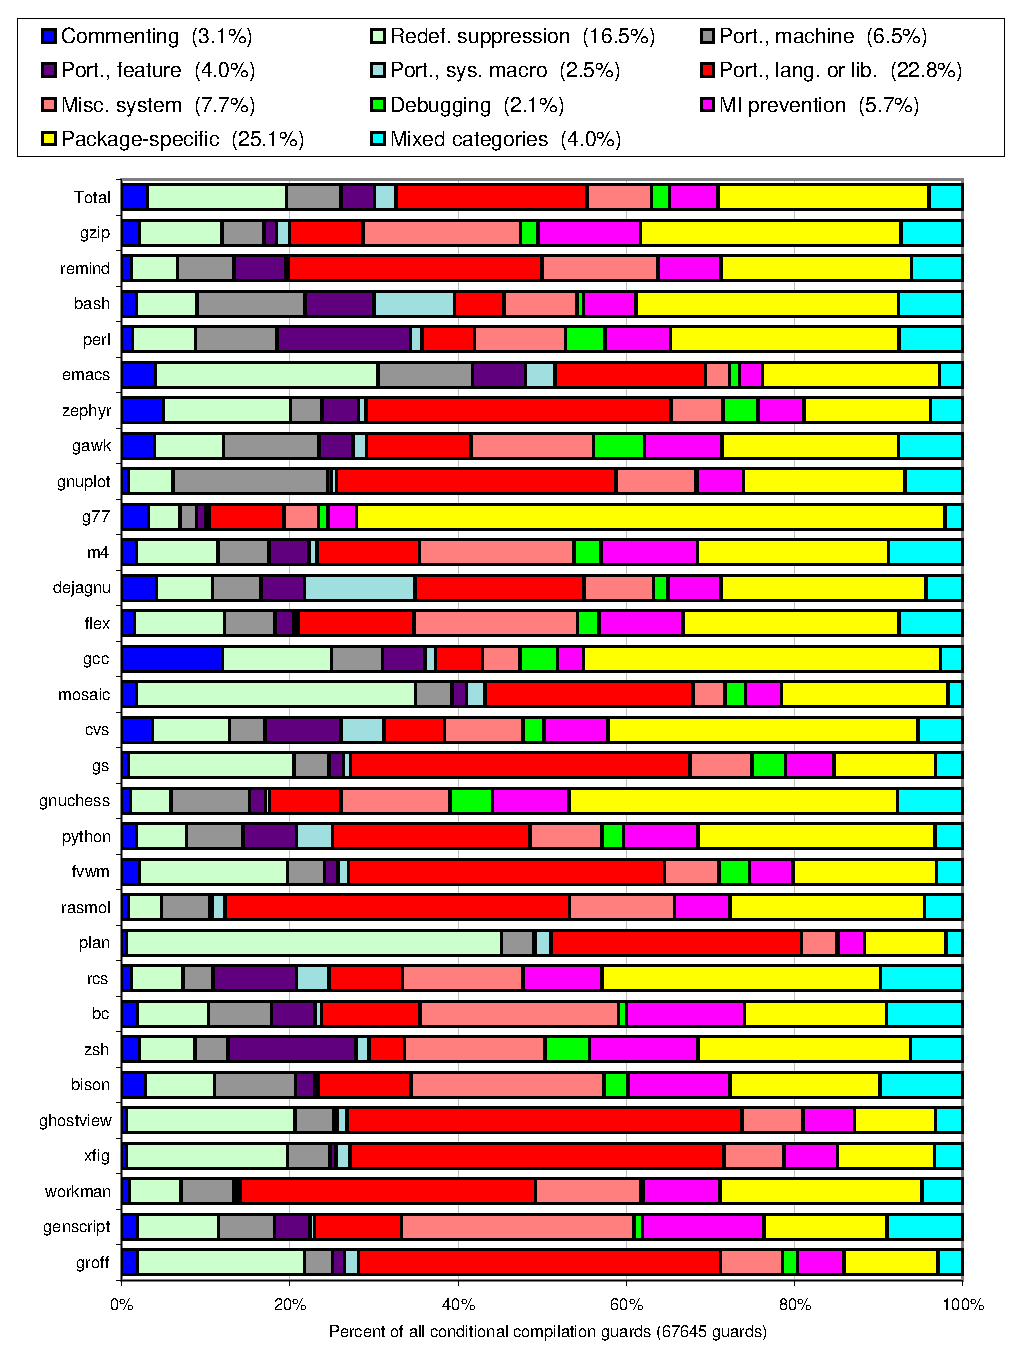
\epsfig{file=fig/ccd-categories.eps,height=6in}}
\captionsmall{Categories for conditional compilation directives.  The
  legend should be read across, by rows.}
\label{fig:ccd-categories}
\end{figure}

Cpp conditionals are used to control inclusion of code for portability,
debugging, efficiency, and other purposes.  The programmer intention behind
a {\tt \#if} line can often be inferred from its structure or context or
the macros it uses.  This classification can reveal the structure of
conditional compilation directives and assist in program understanding.

We categorized each Cpp conditional into one of the categories of
Figure~\ref{fig:ccd-categories} (the categories are described below).  For
conditionals that could not be categorized based on their structure or
context, we classified each macro appearing in the conditional according to
what system properties it reifies.  If each macro in the conditional has the
same classification, then the conditional is given that classification;
otherwise, the conditional is classified as ``mixed usage''.

There is significant variation among packages, and no clear pattern of use
emerges.  Portability accounts for over half of conditional compilation
directives.  Redefinition warning suppression, at 16.5\%, is surprisingly
high; it is essentially a macro definition mechanism, not a conditional
inclusion technique.  Mixed categories are relatively rare.  This suggests
both that the conventions for macro names are fairly standardized and that
programmers rarely write conditional tests that combine entirely different
concerns in a single expression.


Cpp conditionals are classified according to structure or context as follows:
\begin{description}\itemsep 0pt \parskip 0pt
\item[Commenting] These guards either definitely succeed and
  have no effect as written (e.g., \texttt{\#ifdef 1}), or definitely fail
  and unconditionally skip a block (e.g., {\tt \#ifdef (0 \&\&
  \verb|OTHER_TEST|)}).  These guards comment out code or override other
  conditions (e.g., to unconditionally enable a previously experimental
  feature).
      
\item[Redefinition suppression] These guards test non-definedness of
  symbol, and control only a definition of the same symbol, thus avoiding
  preprocessor warnings about a redefinition of a name (e.g.,
  \texttt{\#ifndef FOO} followed by \texttt{\#define FOO ...} and
  \texttt{\#endif}).  
  The purpose is to provide a default value used unless another part of the
  system, or the compilation command, specifies another value.

\end{description}

For Cpp conditionals not classified by the above rules, each macro
appearing in the conditional is placed in one of the following categories:

\begin{description}\itemsep 0pt \parskip 0pt
%% See ccd_lexical_category in em_analyze for the routines
%% which implements these heuristics

\item[Portability, machine]
  These symbols name the operating system or machine
  hardware (e.g., \texttt{sun386} or \texttt{MACINTOSH}).
      
\item[Portability, feature] These symbols describe specific parameters
      or capabilities of the target machine or operating system (e.g.,
      \texttt{BYTEORDER}, \verb|BROKEN_TIOCGWINSZ|).  
      
%      These symbols are different from ``portability, machine'' because
%      they may correspond to multiple machines or architectures.

\item[Portability, system macro]
  These symbols are commonly defined constants or
  pseudo-inline functions in system or language libraries (e.g.,
  \verb|O_CREATE|, \texttt{isalnum}, or \verb|S_IRWXUSR|).

\item[Portability, language or library]
  These symbols are predefined by a compiler, defined by a standard
  library, or defined by the package as part of the build
  process to indicate existence of compiler, language, or library features
  (e.g., \texttt{GNUC}, \texttt{STDC}, or \verb|HAS_BOOL|).

\item[Miscellaneous system]
  These symbols are reserved (they begin with two underscores) and do
  not fit any other category.
      
\item[Debugging]
  These symbols control inclusion of debugging or tracing code.  The macro
  names include \texttt{DEBUG} or \texttt{TRACE} (or both).
      
\item[Multiple inclusion prevention]
  These guards encompass an entire file to ensure that the enclosed code is
  seen only once per translation unit by the compiler.  Such guards are
  indicated by convention with a trailing \verb|_H| or \verb|_INCLUDED| in the macro name
  they check.

\item[Package-specific] 
  These symbols are specific to the given package.  They do not fit any of
  the other categories.

\end{description}

When every macro appearing in a Cpp conditional is classified identically,
the conditional gets that classification, too.  Otherwise, it is classified
as ``mixed'':

\begin{description}\itemsep 0pt \parskip 0pt
\item[Mixed categories] These guards test multiple symbols
      that independently fall into different categories (e.g.,
      {\tt \#if defined(\verb|STDIO_H|) || \verb|SYSV_SIGNALS|}).
\end{description}



% \subsection{Number of arguments}
% 
% \begin{figure}
% \centerline{\epsfig{file=fig/cat-numargs.eps,height=4in}}
% \captionsmall{Is this worth including?
%   [[PROBLEM:  the numbers in this legend don't accord with those in
%   previous legends by name.  This is because the numargs information was
%   gleaned from the .catg file which contains only the macro bodies and
%   the filename they were found in, thus there is no way to include macro
%   bodies defined outside the package of macro names that are defined
%   somewhere inside the package as is the case almost everywhere else;
%   I'm now thinking that this information could've/should've been used
%   for aiding the categorizations: i.e., a null define taking no
%   arguments is a lot different than one taking arguments;  since that
%   wasn't done, I'm inclined to drop this since to avoid the
%   inconsistency in the numbers (and because it is of questionable
%   utility as presented now --gjb]]}
% \label{fig:cat-numargs}
% \end{figure}
% 
% 
% You might wonder whether macros are used like functions (taking arguments)
% or like constants (taking no arguments).  
% [[However, a fair number of statement macros also take no arguments.]]
% We graphed that in
% Figure~\ref{fig:cat-numargs}.  This seems irrelevant to me; I don't see
% where to fit it in, or what to say about it.



\section{Dependences}
\label{sec:dependence}
\label{sec:last-content-section}

Macros control the program that results from running Cpp in two distinct
ways.  {\em Inclusion} dependence results from Cpp conditionals which test
macros (for definedness, or by examining expansions) to determine which
lines of the Cpp input appear in the output.  {\em Expansion} dependence
results from replacement of macros outside Cpp conditionals by their
definition bodies, which controls the content of the lines on which the
macros appear.  This section reports the incidence of these dependences,
both by macro and by line.

We report both direct and indirect dependences.  A line directly depends
upon macros that appear in the line or in a {\tt \#if} condition whose
scope contains the line.  It indirectly depends on macros that control the
definitions of directly controlling macros.  After {\tt \#define
\verb|S_ISBLK|(m) ((m)~\&~\verb|S_IFBLK|)}, the final text of a line that
uses \verb|S_ISBLK| depends not just on its definition but also on that of
\verb|S_IFBLK|.  An indirect dependence is an expansion dependence if every
dependence in the chain is an expansion dependence; otherwise, the indirect
dependence is an inclusion dependence.

We do distinguish must from may dependences.  A must dependence links a use
to the macro's known single definition site; a may dependence links a use
to multiple definition sites, when it is not know which definition is in
effect at the point of use.  When a macro is defined on both branches of a
{\tt \#if} conditional, the macro's definedness does not depend on the
values tested in the conditional, though its value does.  We do track
dependences across file boundaries: if a macro controls whether a file is
{\tt \#include}d, then the macro also controls every line of that file.

%% This makes absolutely no sense.  What is going on here?
%% I think there's something meaningful about lopping off prefixes of must
%% dependences, but can't puzzle it out now.  -MDE 11/1/97
% When different conditions control different definitions of a macro, uses
% are dependent on the independent parts of those conditions.  For instance,
% after
% \begin{verbatim}
%   #if A
%     #if B1
%       #define M ...
%     #elsif B2
%       #define M ...
%     #else
%       #define M ...
%     #endif
%   #endif
% \end{verbatim}
% a use of macro {\tt M} is expansion-dependent on {\tt B1} and {\tt B2}, but
% not on {\tt A}, which must have been set to true in order for {\tt M} to be
% defined at all.  That is, no setting of {\tt A} can affect {\tt M}'s

\begin{figure}
\centerline{\epsfig{file=fig/dep-byline.eps,height=4in}}

\captionsmall{Percentage of lines dependent on a particular number of macros (or
  fewer).  For instance, 93\% of all lines are expansion-dependent on two
  or fewer macros, and 90\% of all lines are inclusion-dependent on 27 or
  fewer macros.  The log scale is shifted by unity in order to place 0
  on the scale:  before plotting, we added 1 to each of the x axis values,
  then relabeled ``1'' as ``0''.}
\label{fig:dep-byline}
\end{figure}


The statistics reported in this section are underestimates because they
omit two packages which aggressively use macros.  The full dependence
information for \pkg{emacs} and \pkg{mosaic} exceeded our computer's
virtual memory, in part due to use of Motif, a complex external library.
(While this paper reports only on macros defined in each package, we
computed dependences and other information for all macros, including those
defined or used in libraries.)  We did generate dependence information for
\pkg{plan}, which is the smallest of the three packages in our test suite
that use the Motif library.


\subsection{Dependences by line}

%%% Figure fig:dep-byline really belongs here, but I'm trying to put it on
%%% a separate page from fig:dep-bymacro.

Figure~\ref{fig:dep-byline} graphs the percentage of lines dependent on a
given number of macros.  Over two in five lines (42\%) are controlled by
macros (this is the complement of the 58\% of lines that depend on zero
macros).  Almost as many lines (38\%) are inclusion-controlled by at least
one macro; some of these lines, such as those in header files, appear
unconditionally but are inside a guard to avoid multiple inclusion.  Over
one in four lines (28\%) expands a macro, a higher value than we
anticipated.

Expansion dependence on multiple macros is not prevalent\,---\,only 5\% of
lines are expansion-dependent on more than 3 macros, and only 1\% are
expansion-dependent on more than 7 macros.  However, one line of
\pkg{gcc}\,---\,{\tt \verb|LEGITIMIZE_ADDRESS| (x, oldx, mode,
win);}\,---\,is expansion-dependent on 187 different macros.  Macro
\verb|LEGITIMIZE_ADDRESS| is defined 30 times in \pkg{gcc}, many of the
definitions dozens of lines long and themselves studded with macro
invocations.  Overall, only 13 out of 325,000 lines in \pkg{gcc} are
expansion-dependent on more than 100 macros.

Inclusion dependences have a much wider distribution.  One in twenty lines
is inclusion-dependent on at least 133 macros, and 1\% of lines are
dependent on over 300 macros.  As an example, the line of \pkg{gcc}
mentioned above has 182 inclusion dependences (with only 13 macros in
common with its set of expansion dependences), but over over 10,000 lines
of \pkg{gcc} have even heavier inclusion dependences than that.

On average, each line in the {\numpackageslesstwo} packages tested is 
expansion-dependent on .04 macros, inclusion-dependent on .31 macros, has
both varieties of dependence on .01 macros, and has some dependence on .34
macros.
      

\subsection{Dependences by macro}

\begin{figure}
% This works, but the figures are upside-down.
% \centerline{\epsfig{file=fig/exp-dep-bymacro.eps,angle=90,height=3.75in}}
% \centerline{\epsfig{file=fig/incl-dep-bymacro.eps,angle=90,height=3.75in}}
% Can't use ``height'' when rotating by -90 or +270; I don't know why.
% \centerline{\epsfig{file=fig/exp-dep-bymacro.eps,angle=270,width=.5\linewidth}}
% \bigskip
% \centerline{\epsfig{file=fig/incl-dep-bymacro.eps,angle=270,width=.5\linewidth}}
\centerline{\epsfig{file=fig/exp-dep-bymacro.eps,angle=270,width=.48\linewidth}%
\ %
\epsfig{file=fig/incl-dep-bymacro.eps,angle=270,width=.48\linewidth}}
\captionsmall{Dependences by macro name for 22648 macro names in 28 packages.
  Each bar represents all macros that control at least as many as the
  labeled percent of the lines in its package (but fewer than the next
  bar).  For instance, the .17 bar in the expansion dependence chart
  indicates that 286 macros each control between .17\% and .26\% of the
  entire package which contains that macro.  The maximum falls in the last
  bucket specified (i.e., the first bucket off the chart is the first empty
  one).  The $\varepsilon$ bar represents a small non-zero value, so that
  macros not controlling any lines are not conflated with macros
  controlling very few lines.  A log scale is used for the x axis.}

%% expansion is red; inclusion is blue
\label{fig:dep-bymacro}
\end{figure}

Figure~\ref{fig:dep-bymacro} graphs how many lines are dependent on each
macro (Figure~\ref{fig:dep-byline} gave the same information by line rather
than by macro).  Since the {\numpackageslesstwo} packages vary in size, the
graphs of Figure~\ref{fig:dep-bymacro} aggregate them by reporting
percentages of a package rather than absolute numbers.

%% The second sentence of this paragraph is a non sequitur.

The expansion dependence chart closely approximates an exponential decay.
Most macros control few lines, a few macros control many lines, and the
transition between the two varieties is gradual.  Most {\tt \#if}
directives (which account for about 2.2\% of all lines) expand at least one
macro; the rare exceptions include testing the compiling machine's
character set.

Of the ten macros that are expanded by more than 5\% of lines in a package,
six are types ({\tt int} and {\tt rtx} in \pkg{gcc}, {\tt ANY} and {\tt
object} in \pkg{python}, {\tt SvANY} in \pkg{perl}, and {\tt const} in
RCS), one is a constant ({\tt NULL} in python), and three are expressions
({\tt ip} in \pkg{workman} and {\tt ArgCount} and {\tt Args} in
\pkg{xfig}).  Three of these ({\tt int}, {\tt const}, and {\tt NULL})
redefine built-in C keywords or values, and those macros are not
necessarily active on every line containing the symbol.  Likewise, {\tt ip}
is an ordinary variable in most of its uses, though our analysis did not
discover that fact.

%         Outliers (> 6\% of all lines expand):
%           int in gcc (14.85\% !)
%           NULL, ANY, object in python
% 
%         Above 5\%: 
%           SvANY in Perl
%           const in RCS
%           ip in workman -- bogus, as defined just twice, then undefined;
%                   most places it is a formal parameter and out of the scope
%                   of the macro definition.
%           ArgCount, Args in xfig (like argc, argv)
%           rtx in gcc (defined to int or int*)
% 
%         Overall, for these top 10:  6 types, 1 constant, 3 expressions



The inclusion dependence graph is bimodal.  While most macros control
inclusion of zero or few lines, quite a few control substantial
fractions (10\% or so) of the package, and there are not a lot of macros in
between.  The graphs for the individual packages exhibit far higher peaks
than the aggregate inclusion dependence graph of
Figure~\ref{fig:dep-bymacro}; summing the graphs tended to average them.
The heaviest dependences are on header files (for instance, \verb|H_PERL|
controls inclusion of over 53\% of \pkg{perl}'s lines).

%        [[It would have been interesting to run these numbers for everything
%          but exclude file multiple inclusion prevention macros.]]


\subsection{Cppp}

Support for multiple dialects of a language is a particularly common use of
the preprocessor, one which leads to unstructured macros (partial
declarations and other difficult-to-handle constructs) and which can be
performed only by the preprocessor, not in the language.  We performed an
experiment to determine whether eliminating these macros would lead to
substantially simpler uses of macros with fewer dependences, failed
classifications of macro bodies, and so forth.

We built a Cpp partial evaluator called Cppp.  Given Cpp-style command-line
arguments specifying which macros are known to be defined or undefined
(and, optionally, their expansions), Cppp discharges Cpp conditionals that
depend on those macros.  Other conditionals, and macro uses, remain in the
output.  Cppp does not expand macros inline or use definitions found in its
input files.

% (It does not eliminate or expand other macros with only one
% remaining definition, because other definitions may appear in libraries or
% on the command line when the package is compiled.)

We used Cppp to preprocess all of our test suite (and all library header
files) with definitions for all the macros that can be depended on if using
ANSI standard C or C++ (including prototypes and booleans) with
POSIX-compliant libraries.  We then reran all of our experiments, but the
results were little changed from the full versions of the packages (which
generally supported both K\&R and ANSI C, and sometimes other dialects as
well): the number of multiple definitions of macros, of failed
classifications, and of dependences on macros did not decline
substantially.  We conclude that macro usage in our test programs presents
no obvious single point of attack: even eliminating one prevalent use did
not eliminate\,---\,or even significantly reduce\,---\,the complexity
introduced by preprocessor.


\section{Related work}
\label{sec:related}

%Split this into:
% * taxonomies
% * checking tools
% * understanding tools such as Emacs hideif mode
% * other?

We could find no other empirical study of the use of the C preprocessor
nor any other macro processor.  However, we did find some guidance on
using C macros effectively, tools for checking macro usage, and
techniques for understanding and exploring C source code that uses the
preprocessor.

A number of organizations provide hints about effective ways to the use the
C preprocessor.  The GNU C preprocessor manual~\cite{cpp-manual} discusses
a set of techniques including simple macros, argument macros, predefined
macros, stringization macros, concatenation macros, and undefining and
redefining macros.  It also identifies a set of ``pitfalls and subtleties
of macros''; these are much like some of the problems our analysis tool
identifies.  Several coding style guides make recommendations on
preprocessor use and on ways to reduce unexpected behavior resulting from
poorly designed constructs~\cite{Stallman97,ellemtel92,Cannon95,Dolenc90}.
Our empirical data might help refine these sets of suggestions.

Carroll and Ellis state that ``almost all uses of macros can be eliminated
from C++ libraries''~\cite[p.~146]{Carroll95}.  They list eight categories
of macro usage and explain how the software engineer can use C++ language
features instead of using the preprocessor.  Our categories focus on actual
use in C programs rather than potential uses in C++ programs.

Spencer and Collyer provide a set of techniques for achieving portability
without using \texttt{\#ifdef}~\cite{SpencerC92}, which they recommend only
for providing default values for macros and preventing multiple inclusion
of header files.  They suggest using standard interfaces, using separate
files instead of merging them with Cpp conditionals, and testing for
specific features instead of machines in conditional compilation
directives, as we do in Section~\ref{sec:ccd}.  They also break down the
uses of \texttt{\#ifdef} in the 21,000 lines of C News.

Krone and Snelting use mathematical concept analysis to determine the
conditional compilation structure of code~\cite{Krone94}.  They determine,
for each line, which preprocessor macros it depends upon, and display that
information in a lattice.  They do not determine how macros depend upon one
another directly, only by their nesting in {\tt \#if}, and the information
conveyed is about the program as a whole.  When the lattice does not have a
grid-like structure, it is possible that the code does not properly
separate concerns.  Section~\ref{sec:ccd} analyzed single compilation
directives that tested multiple incompatible macros using a fixed set of
categories.


%Greg:  describe LCLint methodology and results.  Say exactly what you did
%(i.e., how hard you tried), and what the results were.  Also, that you tried
%on only 20, not all 30, packages, which doesn't include the biggest ones.

A number of tools check whether specific C programs satisfy particular
constraints.  Various lint~\cite{Johnson77} source-code analyzers check
for potentially problematic uses of C, often including the C preprocessor.
Macro errors are usually discovered as a byproduct of macro
expansion\,---\,for instance, by generating an empty statement which causes
lint to issue a warning\,---\,rather than in their own right.

LCLint~\cite{Evans-fse94,Evans:LCLint} allows the programmer to add
annotations that enable more sophisticated checks than many other lint
programs.  LCLint optionally checks function-like macros\,---\,that is,
those which take arguments\,---\,for macro arguments on the left hand
side of assignments, for statements playing the role of expressions, and
for consistent return types.  LCLint's approach is prescriptive:
programmers are encouraged not to use constructs that might be
dangerous, or to change code that contains such constructs.  We ran
LCLint on our set of packages with its macro diagnostics enabled and
found that its diagnostics were too restrictive to allow parsing to
continue after non-trivial macro definitions\,---\,LCLint reported 3184
parse errors and 571 internal bugs when running on the approximately
4000 files in our suite of packages.  Though LCLint's macro rules seem
useful, some user effort in adding fine-grained annotations to the
target source code's macro definitions is required.

%LCLint considers assignment to a macro argument dangerous but does not
%appear to check for assignments to local variables.~\cite[\S
%8]{Evans:LCLint} [[Should we mention these things?  I don't want to seem
%nitpicky or petty, so if we mention this, mention them as differences,
%not as things LCLint does wrong.
%\begin{quote}
%$\ldots$ a parameter to a macro may not be used as the left hand side
%of an assignment expression $\ldots$, a macro definition must be
%syntactically equivalent to a statement $\ldots$ when it is invoked followed by
%a semicolon $\ldots$, the type of the macro body must match the return
%type of the corresponding function $\ldots$~\cite[\S 8]{Evans:LCLint}
%\end{quote}
%That quotation is really easy to nitpick:
%\begin{enumerate}
% \item assignment parameters is fine (just turn into a reference argument) but
%    assignment of non-parameters that aren't at global scope is quite bad.
% \item in x=foo(); we do NOT want foo() to be a statement
% \item a macro doesn't have a single type, but may have many polymorphic types
%\end{enumerate}
%]]

%% FIX: If we could also list the platforms for which each can compile,
%% that would be great, but I doubt the benefit is worth the effort for now.

Check is a C macro checker that detects some instances of multiple
statements, dangling {\tt \#else}, side effects, and precedence errors
using largely lexical checks~\cite{SpulerS92}.  Precedence errors are
performed on macro uses rather than reporting problematic definitions.  The
authors do not report on the effectiveness of the tool in practice or
justify their tradeoffs between techniques that perform parsing and those
that do not.

A limited number of tools do exist to assist software engineers to
understand code with containing Cpp directives.  Emacs~\cite{GNUEmacs19.26}
provides \texttt{hide-ifdef-mode} which enables the programmer to specify
preprocessor variables as explicitly defined or not defined; the mode then
presents a view of the source code corresponding to that configuration,
hiding code that is conditionally unincluded, much like our Cppp tool.
Various language construct ``tagging'' mechanisms (e.g., \texttt{etags} and
\texttt{ctags}) recognize macro definitions and permit tag-aware editors
to move easily from a macro expansion to the various definitions of that
macro name.

Favre suggests that Cpp be expressed in an abstract syntax like that of
other programming languages~\cite{Favre96}.  After a simple semantics (free
of loops and other complicating constructs) is assigned to it, traditional
analyses such as call graph construction, control and data flow analysis,
slicing, and specialization can be performed on it.  The Champollion/APP
environment doesn't support ``the full lexical conventions of the C
language'' nor macros that take parameters, which make up 28\% of macros in
our study.
The Ghinsu slicing tool~\cite{LivadasS94} takes a similar approach, mapping
Cpp constructs\,---\,particularly macro substitution\,---\,to an internal
representation which supports slicing.


%[[ What debugger does this? --11/21/97 gjb]]
% [[ I don't remember, and couldn't find a reference.  -MDE ]]
% Debuggers exist that can call {\tt \#define}d functions.


\section{Making C programs easier to understand}
\label{sec:easier-to-understand}

The combination of C and Cpp makes a source text unnecessarily difficult
to understand.  A good first step is to eliminate Cpp uses where an
equivalent C or C++ construct exists, and to apply tools to explicate
the remaining uses.  Here we discuss a few approaches to reducing the
need for the preprocessor by better changing the state of the art in C
programming, rather than applying tools to a specific source code
artifact.  We do not seriously consider simply eliminating the
preprocessor, for it provides conveniences and functionality not present
in the base language.

Since many of the most problematic uses of Cpp provide portability across
different language dialects or different operating environments,
standardization can obviate many such uses.  Canonicalizing library
function names and calling conventions makes conditional compilation less
necessary and incidentally makes all programs more portable, even those
which have not gone to special effort to achieve portability.  This
proposal moves the responsibility for portability (really, conformance to a
specification) from the application program into the library or operating
system.  

Likewise, one of the most common uses of Cpp macros could be eliminated if
the C language and its dialects had only a single declaration syntax.
Because most C compilers, and all C++ compilers, accept ANSI-style
declarations, support for multiple declaration styles may have outlived its
usefulness.  The ansi2knr tool~\cite{Deutsch90} translates a C program
using ANSI style function declarations into one using classical function
declarations.  This tool frees authors from maintaining two commonly
required configurations.

Some Cpp directives, such as {\tt \#include}, can be moved into the
language proper; this would also eliminate the need for Cpp constructs that
prevent multiple inclusion of header files.  Likewise, compilers that do a
good job of constant-folding and dead code elimination can encourage
programmers to use language constructs rather than relying on the
guarantees of an extra-linguistic tool like Cpp.  It is less important that
compilers perform the appropriate optimizations than that programmers have
confidence in this; skeptical programmers will prevent code from being
generated by using Cpp to hide computations from the compiler.

Common Cpp constructs could be replaced by a special-purpose syntax.  For
instance, declarations or partial declarations could be made explicit
objects; similar support could be provided for repetitive constructs and
dynamic scoping.  Manipulations of these objects would then be performed
through a clearly-specified interface rather than via string and token
concatenation, easing the understanding burden on the programmer or tool.
Such uses would also be visible to the compiler and to program checkers
such as lint.  The downside of this approach is the introduction of a new
syntax or new library functions which may not simplify the program text and
which cannot cover every possible case.

Some macro systems have been designed that avoid particular pitfalls of Cpp.
A hygienic macro system~\cite{lfp86*151} never unintentionally captures
variables, though it can do so when necessary via a special construct.
Other macro systems require that their output to be a syntactic AST rather
than merely a token stream~\cite{WeiseC93}.

An alternative approach which avoids the clumsiness of a separate language
of limited expressiveness is to make the macro language more
powerful\,---\,perhaps even using the language itself via constructs
evaluated at compile time rather than run time.  (The macro systems of
Common Lisp~\cite{commonlisp:languagespec} and
Scheme~\cite{Clinger91:R4RS}, and their descendants~\cite{WeiseC93}, take
this approach.)  In the limit, a language can provide a full-fledged
reflection capability~\cite{kicz91}.  Such an approach is highly general,
powerful, and theoretically clean.  The added generality, however, degrades
a tool's ability to reason about the source code.  In practice, such
systems are used in fairly restricted ways, perhaps because other uses
would be too complicated.  A dialogue among users, compiler writers, tool
writers, and language theorists is necessary when introducing a feature in
order to prevent unforeseen consequences from turning it into a burden.



\section{Conclusions}
\label{sec:conclusion}

% [[Grist for conclusion: These data demonstrate that multiple definitions of
% symbols is not numerically frequent; even more importantly, the definitions
% of a symbol tend to be compatible, as shown in
% Section~\ref{sec:inconsistent}.]]


% \subsection{Relevance of the results}

The results of this research are of interest to language designers, tool
writers, programmers, and software engineers.

Language designers can examine how programmers use the macro system's
extra-linguistic capabilities.  Future language specifications can
directly support (or prevent!)\ such practices thus imposing greater
discipline and structure.

% [[[Think more about this:  Also, how do language choices lead to more/less
% tightly integrated (as opposed to open, component-based) environments?
% E.G., no need for \verb|__LINE__| in Java?]]]

Programming tool writers can choose to cope only with common uses of the
preprocessor.  By partial preprocessing (or embedded understanding of
some Cpp constructs), a parser can maintain the
programmer-oriented abstractions provided by preprocessor directives and
macro names while not getting confused by non-syntactic programs.

Our analyses are of interest to programmers who wish to make their code
cleaner and more portable.  By recognizing the widely-used Cpp idioms,
programmers can choose to limit their use of the preprocessor to
constructs that other tools are most likely to cope with easily.  They
can choose to avoid constructs that cause tools (such as test frameworks
and program understanding tools) to give incomplete or incorrect
results.

% Also, learn weird new Cpp tricks!

Finally, our results are of interest to software engineers for all of the
above reasons and more.  Since this is the first study of Cpp usage of
which we are aware, it is worth performing simply to determine whether the
results were predictable a priori; in addition, we found
some interesting, and in some cases surprising, features of our suite of
programs.


%% See slide 15 and its notes from Mike's quals talk.
% \subsection{Future work}
 
These results suggest a wide variety of future avenues for research, both
in terms of expanding our understanding of uses of the preprocessor in
practice and in addressing the issues identified by this study.

We did not analyze any libraries (e.g., \pkg{glibc}) for their macro use
patterns.  Comparing how Cpp use in libraries and application code may
yield insights into the different needs of library authors.  Other
comparisons, such as Unix vs.~Microsoft Windows packages, may also prove
valuable.

We did not formally analyze any C++ source code.  Preliminary results
indicate that many C++ packages rely heavily on Cpp, even when C++ supports
a nearly identical language construct.  This unfortunate situation probably
stems from a combination of trivial translations from C to C++ and of C
programmers becoming C++ programmers without changing their habits.  A
useful analysis of C++ packages would consider the code in the context of
both the history of the package and the background of its authors.

Further analysis of the macros with free variables is needed to see which
of the roughly 32\% of expression macros should be easy to convert to
inline functions.  In particular, we did not investigate whether the free
variables in macro definitions referred to local or global variables.  The
former achieve dynamic scoping which is impossible using the C language
proper, while the latter could likely be converted to inline functions.

Our framework currently does not benefit from analyzing the context of
macro expansions in determining a macro's category.  For example, a
macro used where a type should appear can be inferred to expand to a
type; a macro used before a function body is probably expanding to a
declarator.

Additionally, the framework is overly conservative with respect to
conflicting definitions.  We assume that every occurrence (except in
strings and comments) of any name that is \texttt{\#define}d is a macro
use and could correspond to any of the definitions of that same name.
This pessimism provides an upper bound on the preprocessor complexity of
the source code, but is too inaccurate when considering code
modifications.  We currently are experimenting with a different
framework that accurately tracks macro definitions and uses to provide
support for more sophisticated reasoning and code transformations.

\section*{Acknowledgments}

This work was supported by a National Science Foundation Graduate
Fellowship and an IBM Cooperative Fellowship.
    
% Any opinions, findings, conclusions, or recommendations expressed in
% this publication are those of the author, and do not necessarily
% reflect the views of the National Science Foundation.


% Not really right:  Don't want the ``References'' section head to be small.
{\small \bibliography{evil}}


\appendix

\section{Merging categories}
\label{app:category-lub}

The following rules determine how two macro definition categories are
merged.  These rules are used when combining categories of multiple
definitions of a symbol in order to assign a category for that macro name,
as in Sections~\ref{sec:mult-def}--\ref{sec:inconsistent}.

\begin{itemize}\itemsep 0pt \parskip 0pt

\item If the categories are the same, use that.

\item If one is an unknown symbol (or the name of an undefined macro), use
  the other on the theory that the unseen definitions are likely to be
  similar to the present one, which is true for well-behaved macros.

\item If one is a null define, use the other.  For instance, a type
  modifier may be present or absent.  In order to either perform an action
  or do nothing, macros not uncommonly expand to either a statement or to
  nothing (though it would be more robust to expand to a null statement in
  the latter case).  Additionally, a macro used as a boolean variable which
  is checked for definedness may be set via a null define or by being
  assigned a constant (generally 1).  This practice is an error if the
  macro is used outside the Cpp {\tt defined} operator, but is also frequent
  and generally innocuous.

\item If one is a constant and the other is an expression, use the latter.

\item If one is an ambiguous list of space-separated symbols and the other
  is reserved word or type, use the latter.  Sequences of symbols can often
  not be definitely identified in isolation, but the other definitions of
  the same name indicate the intended usage.

\item If one is an expression or constant and the other is a semicolonless
  statement, use the latter, for a semicolon can be added to any expression
  to make a statement.  In particular, function calls are classified as
  expressions but may be intended to be used for side effect rather than
  for value.

\item If one is statement-related, use the other if it is the corresponding
  plural form; if both are partial statements, select the more incomplete
  statement category.  (See page~\pageref{item:statement-category} for
  details.)

\item Otherwise, return failure.
\end{itemize}


\end{document}
